\documentclass{beamer}
% \documentclass[handout]{beamer}
\usepackage{pgfpages}
% \setbeameroption{show notes on second screen=right}
% \setbeameroption{show notes}

\usepackage[english]{babel} 
\usepackage[utf8]{inputenc} 

% Gráficos
\usepackage{tikz}
\usepackage{graphicx}
\newlength{\figuresheight}
\setlength{\figuresheight}{7cm}
\setkeys{Gin}{totalheight=\figuresheight,keepaspectratio=true}
\graphicspath{{./images/bmps/}{./images/vects/}{./images/}}
\usepackage{ifpdf}
\ifpdf
  \DeclareGraphicsExtensions{.pdf,.mps,.png,.jpg}
\else
  \DeclareGraphicsExtensions{.eps,.mps}
\fi
\graphicspath{{./images/bmps/}{./images/vects/}{./images/}
  {./images/presentation/bmps/}{./images/presentation/vects/}{./images/presentation/}
  {./images/chapter00/bmps/}{./images/chapter00/vects/}{./images/chapter00/}
  {./images/chapter01/bmps/}{./images/chapter01/vects/}{./images/chapter01/}
  {./images/chapter02/bmps/}{./images/chapter02/vects/}{./images/chapter02/}
  {./images/chapter03/bmps/}{./images/chapter03/vects/}{./images/chapter03/}
  {./images/chapter04/bmps/}{./images/chapter04/vects/}{./images/chapter04/}
  {./images/chapter05/bmps/}{./images/chapter05/vects/}{./images/chapter05/}
  {./images/chapter06/bmps/}{./images/chapter06/vects/}{./images/chapter06/}
  {./images/chapter07/bmps/}{./images/chapter07/vects/}{./images/chapter07/}
}

\usepackage{epsfig}
\usepackage{tabularx}
\usepackage{graphicx}
\usepackage{caption}
\usepackage{subcaption}
\usepackage{pdflscape}
\usepackage{textpos}
\usepackage{fancybox}

\usepackage{amssymb}% http://ctan.org/pkg/amssymb
\usepackage{pifont}% http://ctan.org/pkg/pifont
\newcommand{\cmark}{\ding{51}}%
\newcommand{\xmark}{\ding{55}}%

\usepackage[style=authoryear,natbib=true]{biblatex}
\setbeamertemplate{bibliography item}[text]
\addbibresource{references.bib}


% for downsampling large images
\ifnum\pdfshellescape=1
% Yes, enabled
% #2 is the filename - assumed relative
% IFP - image file path
% IFN - image filename only
% here resizing at 800 px wide
\let\Oldincludegraphics\includegraphics
\newread\myinput
% must add default argument [] so typeout works
\renewcommand\includegraphics[2][\@empty]{%
% debug - print arguments to stdout:
\immediate\message{== #1 ==}
\immediate\typeout{== #2 ==}
% run downsampling bash script
\immediate\write18{mkdir -p downsampled; IFP=#2 ; %
echo "Processing $IFP" ; %
IFN=$(basename $IFP) ; %
echo "downsampled/$IFN" > tmpname ; %
if [ ! -f downsampled/$IFN ]; then %
echo "File downsampled/$IFN not found! Converting..." ; %
% convert $IFP -resize 50\% downsampled/$IFN ; %
convert $IFP -resize 100x downsampled/$IFN ; %
else %
echo "Found downsampled/$IFN - reusing." ; %
fi ; %
} % end write18
% here we should have downsampled file
% retrieve downsample filename first
\immediate\openin\myinput=tmpname
% The group localizes the change to \endlinechar
\bgroup
  \endlinechar=-1
  \immediate\read\myinput to \localline
  % Since everything in the group is local, we have to explicitly make the
  % assignment global
  \global\let\myTmpFileName\localline
\egroup
\immediate\closein\myinput
\immediate\typeout{== \myTmpFileName .. #1 ==}
% Clean up after ourselves
% \immediate\write18{rm -f -- tmpname}
% finally, include downsampled image
\Oldincludegraphics[#1]{\myTmpFileName}
} % end renewcommand
\else
% No, disabled
\fi


\title{Obstacle Detection and Planning for Autonomous Vehicles based on Computer Vision Techniques}
\author{Néstor Morales Hernández} 
\institute{Departamento de Ingeniería Informática \\ Universidad de La Laguna}
\date{June 2014}

\usetheme{Warsaw}

% Berkeley *

% Copenhagen *
% Hannover
% Madrid
% Malmoe
% PaloAlto
% Warsaw

\usepackage{BeamerColor}
\definecolor{mainColor}{rgb}{.125,.7,.25}
\usecolortheme[named=ForestGreen]{structure}

% NOTE: Background
% \setbeamertemplate{background canvas}{\begin{tikzpicture}\node[opacity=.2]{\includegraphics[height=\paperheight]{background}};\end{tikzpicture}}

% \setbeamercolor{alerted text}{fg=orange}
% \setbeamercolor{background canvas}{bg=green}
% \setbeamercolor{block body alerted}{bg=normal text.bg!90!black}
% \setbeamercolor{block body}{bg=normal text.bg!90!black}
% \setbeamercolor{block body example}{bg=normal text.bg!90!black}
% \setbeamercolor{block title alerted}{use={normal text,alerted text},fg=alerted text.fg!75!normal text.fg,bg=normal text.bg!75!black}
% \setbeamercolor{block title}{bg=blue}
% \setbeamercolor{block title example}{use={normal text,example text},fg=example text.fg!75!normal text.fg,bg=normal text.bg!75!black}
% \setbeamercolor{fine separation line}{}
% \setbeamercolor{frametitle}{fg=brown}
% \setbeamercolor{item projected}{fg=black}
% \setbeamercolor{normal text}{bg=black,fg=yellow}
% \setbeamercolor{palette sidebar primary}{use=normal text,fg=normal text.fg}
% \setbeamercolor{palette sidebar quaternary}{use=structure,fg=structure.fg}
% \setbeamercolor{palette sidebar secondary}{use=structure,fg=structure.fg}
% \setbeamercolor{palette sidebar tertiary}{use=normal text,fg=normal text.fg}
% \setbeamercolor{section in sidebar}{fg=brown}
% \setbeamercolor{section in sidebar shaded}{fg=gray}
% \setbeamercolor{separation line}{}
% \setbeamercolor{sidebar}{bg=red}
% \setbeamercolor{sidebar}{parent=palette primary}
% \setbeamercolor{structure}{bg=black, fg=green}
% \setbeamercolor{subsection in sidebar}{fg=brown}
% \setbeamercolor{subsection in sidebar shaded}{fg=gray}
% \setbeamercolor{title}{fg=brown}
% \setbeamercolor{titlelike}{fg=brown}

%% Video stuff
\usepackage{movie15}

% \AtBeginSubsection[]
% {
%   \begin{frame}
%     \frametitle{Table of Contents}
%     \tiny
%     \tableofcontents[currentsection]
%   \end{frame}
% }

\begin{document}
\addtobeamertemplate{headline}{}{%
\begin{textblock*}{100mm}(0.02cm,-0.8cm)

\includegraphics[height=.7cm]{verdino}
\end{textblock*}}

  \begin{frame}[plain]
    \centering
    
%     \includegraphics[height=0.5cm]{ull} \hspace*{0.5\textwidth}
%     
\includegraphics[height=2cm]{verdino} 
%     \begin{textblock*}{100mm}(0.02cm,-0.8cm)
%       
\includegraphics[height=.7cm]{verdino}
%     \end{textblock*}

    \titlepage
    
    \tiny
    \hfill Under the guidance of:\\
    \scriptsize
    \hfill Leopoldo Acosta Sánchez\\
    \hfill Jonay T. Toledo Carrillo

  \end{frame}

% \graphicspath{{./images/bmps/}{./images/vects/}{./images/}
  {./images/presentation/bmps/}{./images/presentation/vects/}{./images/presentation/}
  {./images/chapter00/bmps/}{./images/chapter00/vects/}{./images/chapter00/}
  {./images/chapter01/bmps/}{./images/chapter01/vects/}{./images/chapter01/}
  {./images/chapter02/bmps/}{./images/chapter02/vects/}{./images/chapter02/}
  {./images/chapter03/bmps/}{./images/chapter03/vects/}{./images/chapter03/}
  {./images/chapter04/bmps/}{./images/chapter04/vects/}{./images/chapter04/}
  {./images/chapter05/bmps/}{./images/chapter05/vects/}{./images/chapter05/}
  {./images/chapter06/bmps/}{./images/chapter06/vects/}{./images/chapter06/}
  {./images/chapter07/bmps/}{./images/chapter07/vects/}{./images/chapter07/}
}

\section{Introduction}
  \begin{frame}{Introduction}
    \begin{itemize}
      \item<1-> Humans should not drive.
      \begin{itemize}
	\item<2-> Road injuries are one of the top-ten causes death, according to the World Health Organization (WHO).
	\note {Fortunately, the number of deaths for this cause has been reduced.}
	\note {Popularization of Advanced Driver Assistance Systems (ADAS) could be very related to this fact.}
	\item<3-> Driving is difficult, too.
	\note{An average US citizen expends 38 hours stuck in traffic.}
      \end{itemize}
      \item<4-> The amount of research related to autonomous vehicles has increased a lot.
    \end{itemize}  
    \begin{center}
      \includegraphics<1-1>[height=.5\textheight]{CarCartoon}
      \includegraphics<2-2>[height=.5\textheight]{WHO-data-10-deaths}
      \includegraphics<3-3>[height=.5\textheight]{trafficsigns}
      \includegraphics<4-4>[height=.5\textheight]{uav_research}
    \end{center}
  \end{frame}
  
  \begin{frame}{Advantages of autonomous vehicles}
    \begin{columns}[c] % the "c" option specifies center vertical alignment
      \column{.5\textwidth} % column designated by a command
      \begin{itemize}
	\item<1-> Higher safety.      
	\item<2-> Reduced traffic congestion.
	\item<3-> More free time.
	\item<4-> Higher speed limits.
	\item<5-> Occupant constraints.
	\item<6-> Parking problems.
	\item<7-> Traffic police.
	\item<8-> Vehicle insurance.
	\item<9-> Road signs.
	\item<10-> Smoother ride.
      \end{itemize}  
      \column{.5\textwidth}
      \begin{center}
	\includegraphics<1-1>[width=\textwidth]{safety}
	\includegraphics<2-2>[width=\textwidth]{congestion}
	\includegraphics<3-3>[width=\textwidth]{freetime}
	\includegraphics<4-4>[width=\textwidth]{speedlimit}
	\includegraphics<5-5>[width=\textwidth]{stpatricks}
	\includegraphics<6-6>[width=\textwidth]{parking}
	\includegraphics<7-7>[width=\textwidth]{police}
	\includegraphics<8-8>[width=\textwidth]{insurance}
	\includegraphics<9-9>[width=\textwidth]{roadsign}
	\includegraphics<10-10>[width=0.8\textwidth]{smoothride}
      \end{center}
    \end{columns}
    
    \note {
    \begin{itemize}
      \item As said, higher safety due a to a decrease in the number of traffic accidents.
      \item Reduced traffic congestion, as the roads can increase their capacity.
      \item Vehicle occupants can spend their time in things other than driving.
      \item Higher speed limits.
      \item Occupants are not tied to constraints like being under age, blind, intoxicated, etc.
      \item Alleviation of parking scarcity and reduction of space required for vehicle parking.
      \item Reduction in the need for traffic police and vehicle insurance.
      \item Physical road signs will not be needed anymore: autonomous cars could receive necessary communication electronically.
      \item Smoother ride.
    \end{itemize}
    }
  \end{frame}

  \subsection{Problem Statement}
  \begin{frame}{Problem Statement}
    \begin{itemize}
     \item<1-> We propose different methods which will be used for the detection and tracking of obstacles by our prototype, Verdino.
     \item<2-> These will be used by a global and a local planner for generating and following a safe path.
    \end{itemize}
    \begin{center}
      \includegraphics<1->[height=.4\columnwidth]{verdino}
    \end{center}
  \end{frame}
  
  \begin{frame}{Pipeline}
    \begin{center}
      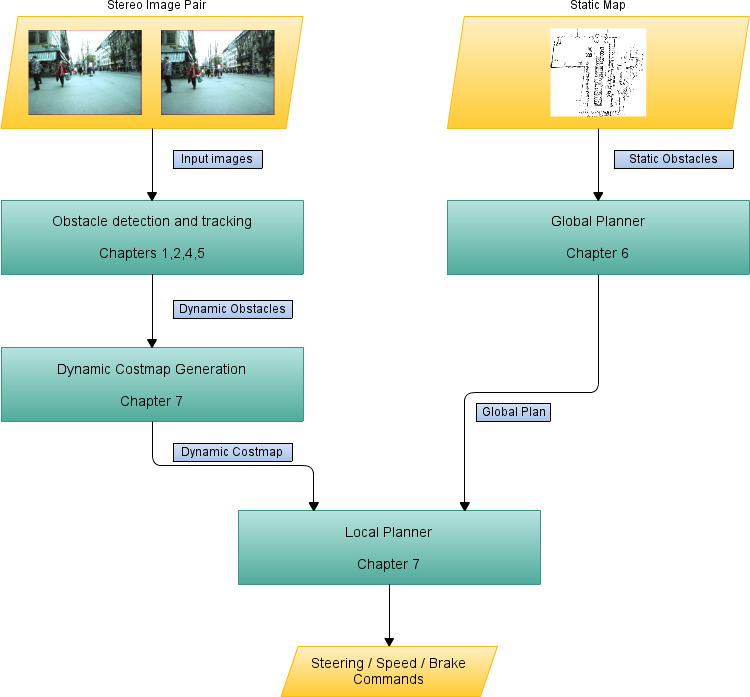
\includegraphics{pipeline_cp0}
    \end{center}
    
  \end{frame}

  
  \begin{frame}{Obstacle detection and tracking}
    \begin{itemize}
    \item<1-> Goals:
      \begin{enumerate}
      \item<2-> Good obstacle detection rate. 
      \item<3-> Obstacle localization.
      \item<4-> Real time.
      \item<5-> Environment conditions independence.
      \item<6-> Tracking capabilities.
      \item<7-> Moving cameras.
      \end{enumerate}
    \end{itemize}
  \end{frame}
  
  \begin{frame}{Obstacle detection and tracking}
    \begin{itemize}
      \item <1-> We propose four different approaches:
      \begin{enumerate}
	\item<1-> Change detection and image registration. 
	\item<2-> Background substraction and nonrigid point set registration.
	\item<3-> Stixels.
	\item<4-> Voxels and a particle filter.
      \end{enumerate}
    \end{itemize}
      
    \begin{center}
      \includegraphics<1-1>[height=.3\columnwidth]{database}
      \includegraphics<2-2>[height=.3\columnwidth]{fig6}
      \includegraphics<3-3>[height=.3\columnwidth]{stixels_over_original}
      \includegraphics<4-4>[height=.3\columnwidth]{fakePointCloud}
    \end{center}
  \end{frame}
  
  \begin{frame}{Obstacle Avoidance and Planning}
    We distinguish two different levels:
    \begin{enumerate}
     \item<1-> Global planning. 
     \item<2-> Local planning.
    \end{enumerate}

    \begin{center}
      \includegraphics<1-1>[height=.35\columnwidth]{figure7}
      \includegraphics<2-2>[height=.35\columnwidth]{example3a}
    \end{center}
  \end{frame}
  
  \begin{frame}{Evaluation of Stereo 3D Reconstruction Algorithms}
    Apart from the previous, we developed some methods intended to assess the performance of the 3D stereo reconstruction algorithms used for the particle filter based approach.
    
    \begin{center}
      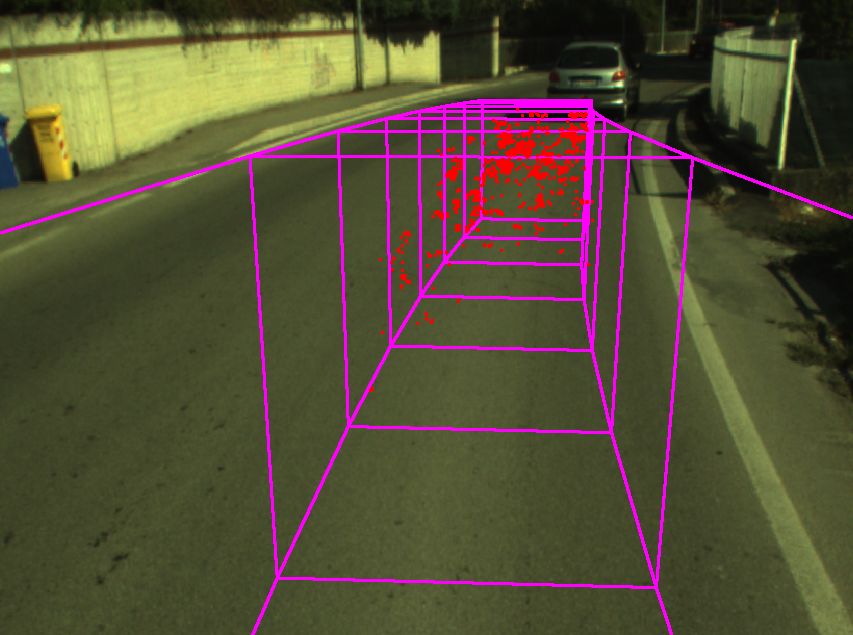
\includegraphics[height=.4\columnwidth]{fc}
    \end{center}
    
  \end{frame}
    
  \subsection{Previous Work}
  \begin{frame}{Autonomous vehicles review}
    \begin{columns}[T] % the "c" option specifies center vertical alignment
      \column{.5\textwidth} % column designated by a command
      \footnotesize
      \begin{itemize}
	\item<1-> \textbf{(1987-1995)} EC EUREKA Prometheus Project.
	\item<2-> \textbf{(1996)} ARGO Project.
	\item<3-> \textbf{(2004)} $1^{st}$ DARPA's Grand Challenge.
	\item<4-> \textbf{(2005)} $2^{nd}$ DARPA's Grand Challenge.
	\item<5-> \textbf{(2007)} DARPA's Urban Challenge.
	\item<6-> \textbf{(2010, 2012, 2013)} Korean Autonomous Vehicle Competition (AVC).
      \end{itemize}  
      \column{.5\textwidth}
      \begin{center}
	\vskip -1cm
       	\begin{overlayarea}{\textwidth}{\textheight}
	  \only<1>{
	  \begin{block}{EC EUREKA Project}
	    \begin{itemize}
	    \item VITA-2\\
	    \begin{center}\includegraphics<1->[width=0.5\textwidth]{vita2}\end{center}
	    \item VaMP\\
	    \begin{center}\includegraphics<1->[width=0.5\textwidth]{VaMP}\end{center}
	    \end{itemize}
	  \end{block}
	  }
	  \only<2>{
	  \begin{block}{ARGO Project}
	    \begin{itemize}
	      \item Lancia Thema.
	      \item Follow the lane marks of a road.
	      \item 1,900\,km
	      \item Average of 60\,Km/h.
	    \end{itemize}
	    \begin{center}\includegraphics<1->[width=0.5\textwidth]{argo}\end{center}
	  \end{block}
	  }
	  \only<3>{
	  \begin{block}{$1^{st}$ DARPA's Grand Challenge}
	    \begin{itemize}
	      \item Mojave Desert.
	      \item 240\,km route.
	      \item Listing of check points.
	      \item None finished the route.
	    \end{itemize}
	    \begin{center}\includegraphics<1->[width=0.5\textwidth]{urbanchallenge2004}\end{center}
	  \end{block}
	  }
	  \only<4>{
	  \begin{block}{$2^{nd}$ DARPA's Grand Challenge}
	    \begin{figure}[t]
		    \centering
		    \begin{subfigure}[b]{0.4\textwidth}
		      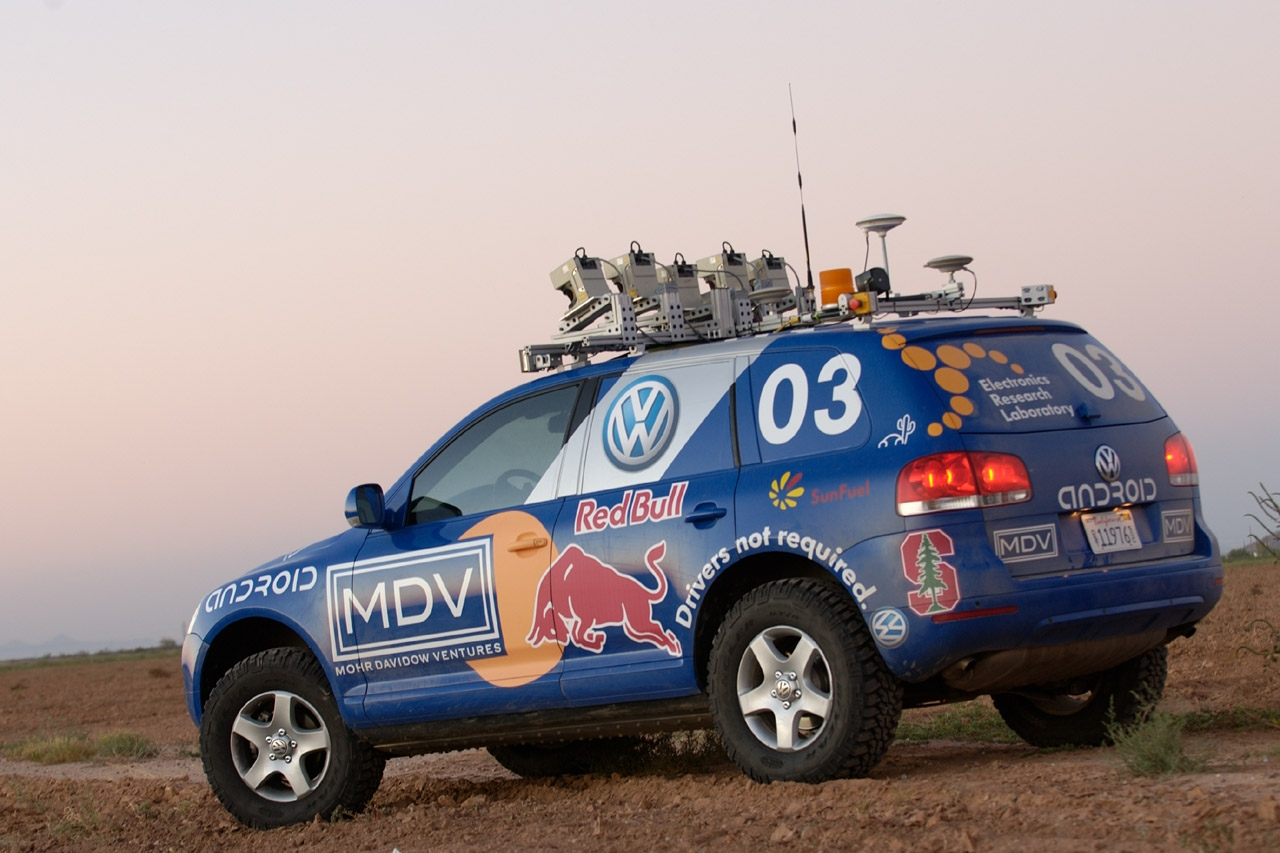
\includegraphics[width=\textwidth]{stanley}
		    \end{subfigure}
		    ~
		    \begin{subfigure}[b]{0.4\textwidth}
		      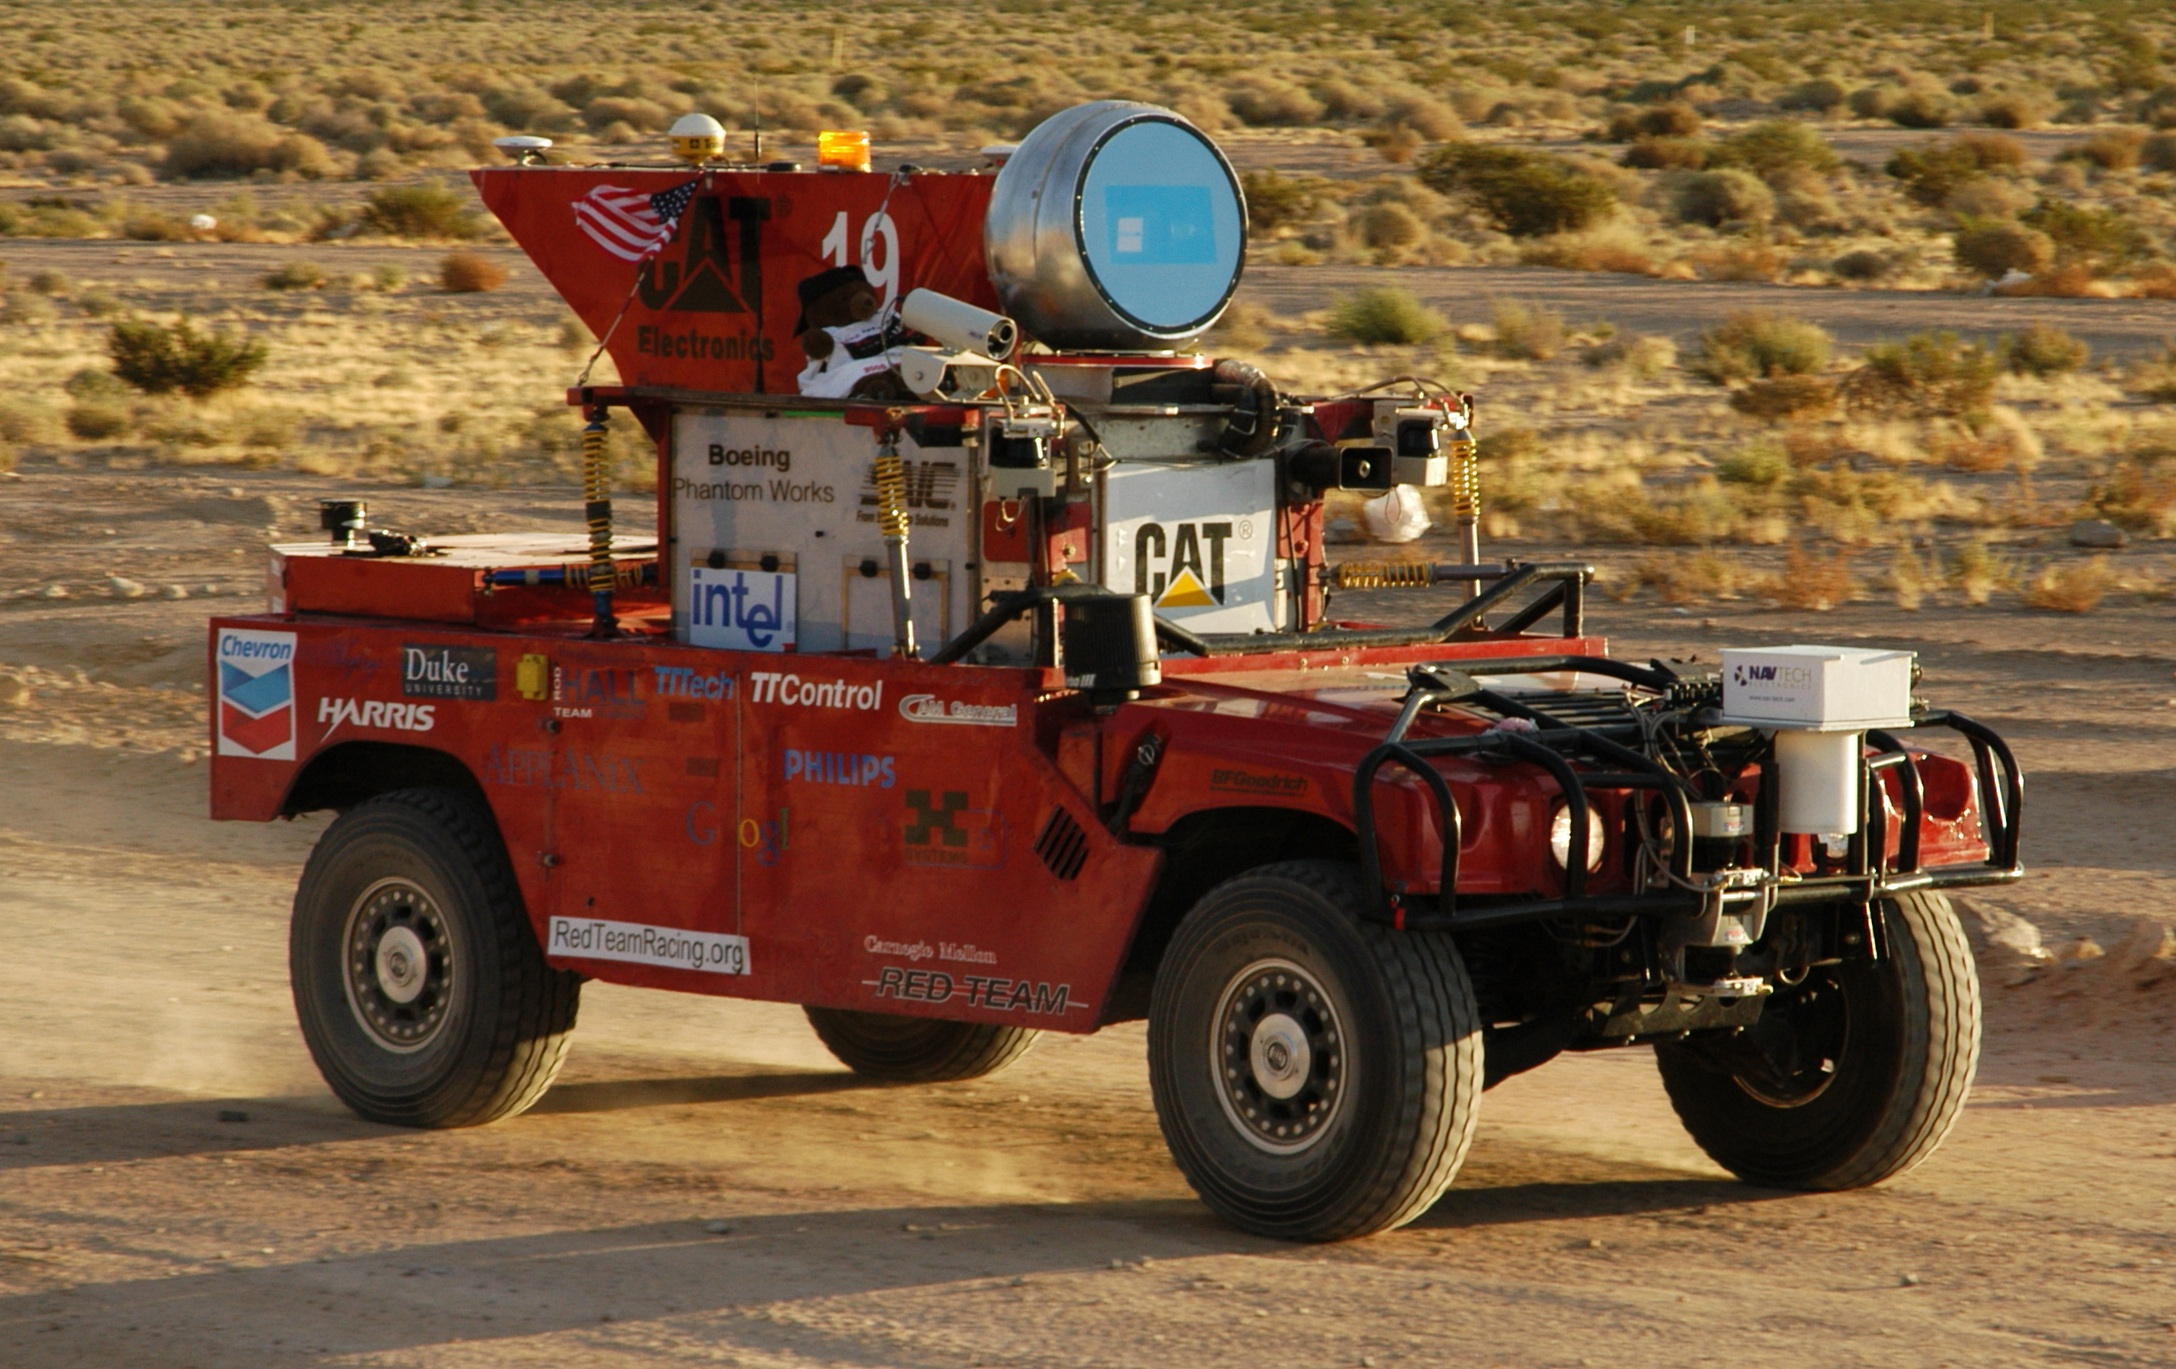
\includegraphics[width=\textwidth]{Sandstorm}
		    \end{subfigure}
		    \\~\\
		    \begin{subfigure}[b]{0.4\textwidth}
		      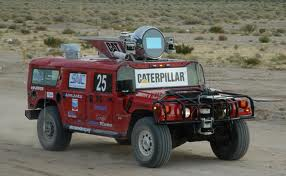
\includegraphics[width=\textwidth]{h1ghlander}
		    \end{subfigure}
		    ~
		    \begin{subfigure}[b]{0.4\textwidth}
		      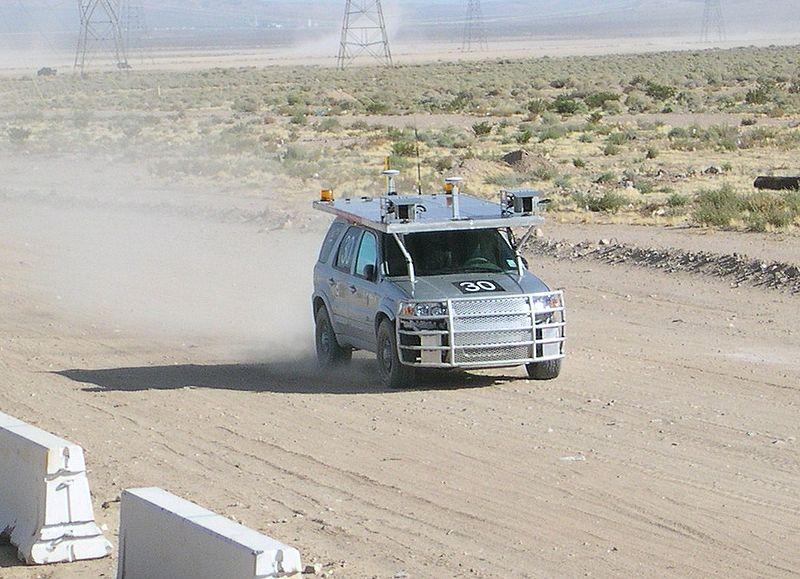
\includegraphics[width=\textwidth]{kat5}
		    \end{subfigure}
		    \\~\\
		    \begin{subfigure}[b]{0.4\textwidth}
		      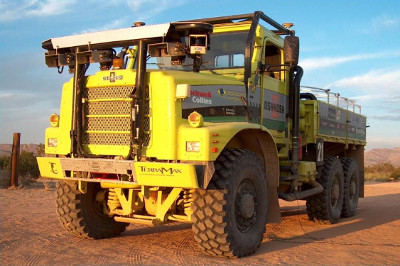
\includegraphics[width=\textwidth]{terramax}
		    \end{subfigure}
	    \end{figure}
	  \end{block}
	  }
	  \only<5>{
	  \begin{block}{DARPA's Urban Challenge}
	    \begin{figure}[t]
		    \centering
		    \begin{subfigure}[b]{0.4\textwidth}
		      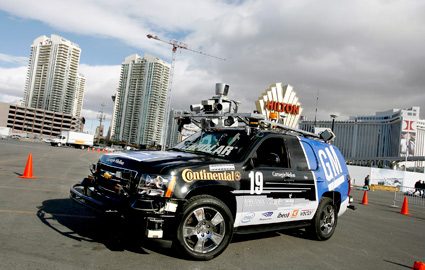
\includegraphics[width=\textwidth]{boss}
		    \end{subfigure}
		    ~
		    \begin{subfigure}[b]{0.4\textwidth}
		      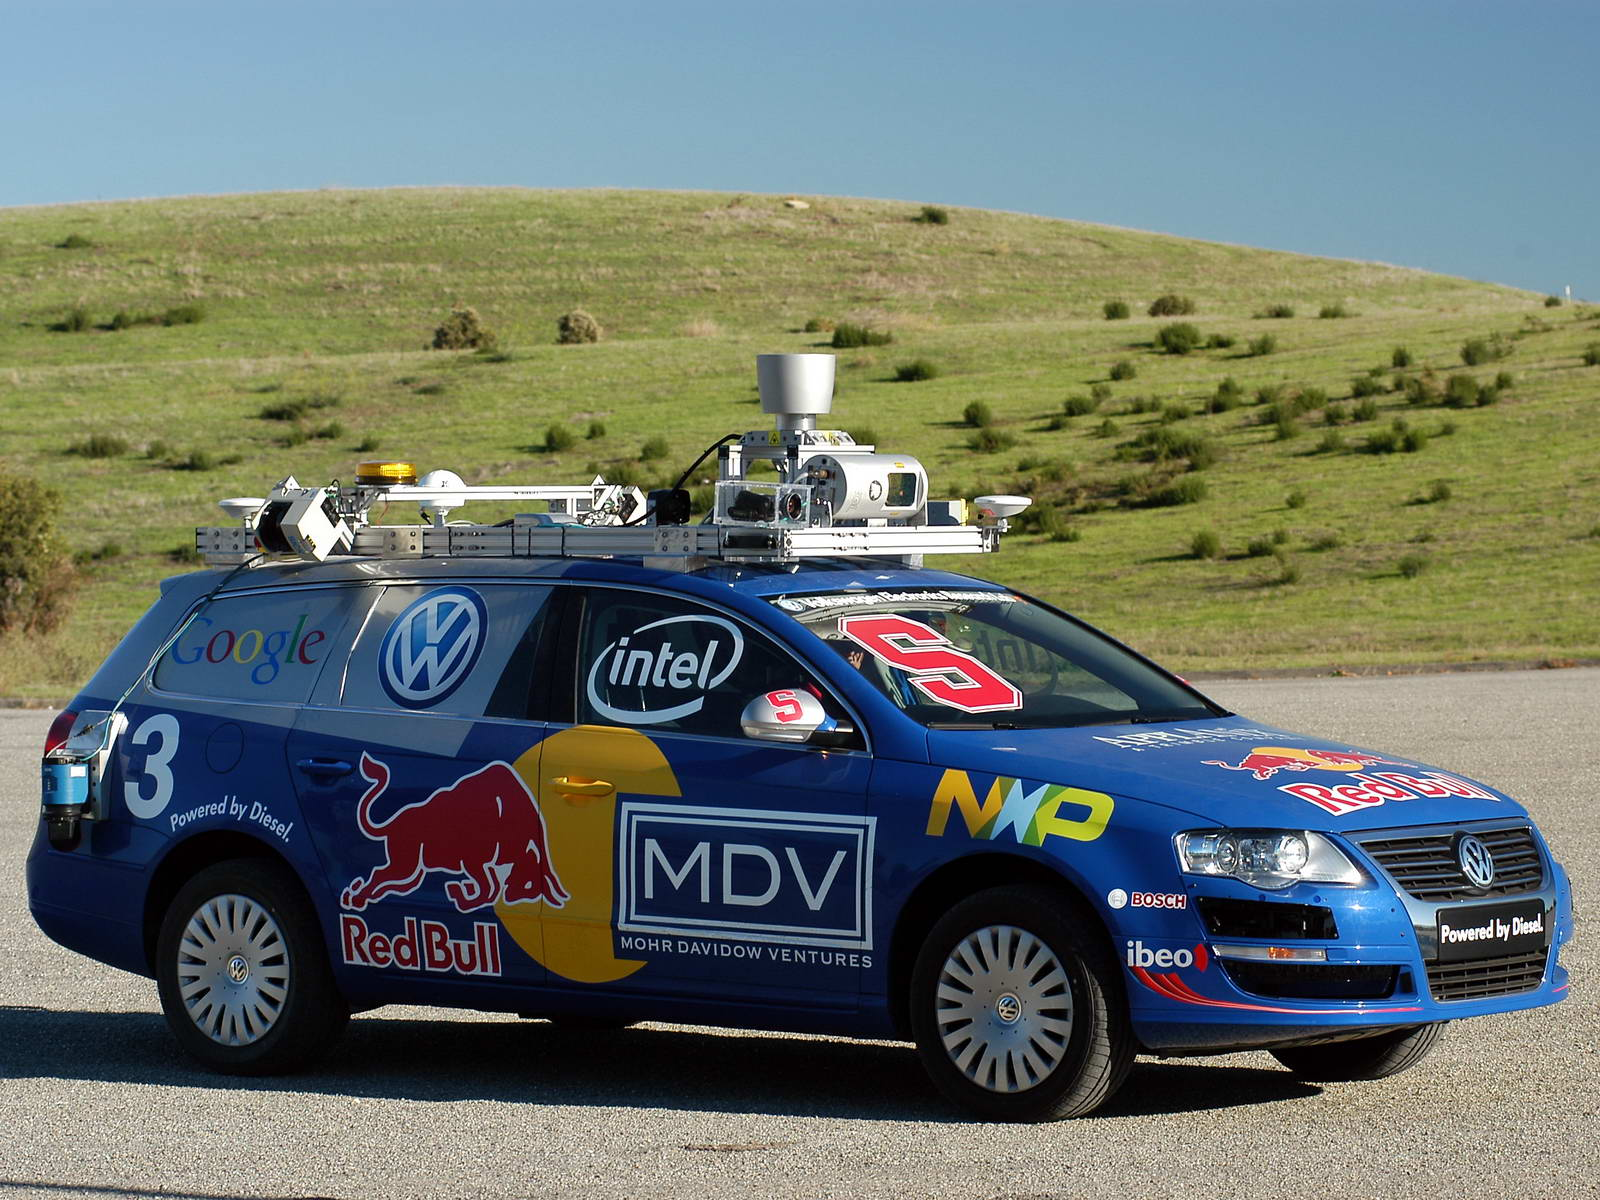
\includegraphics[width=\textwidth]{junior}
		    \end{subfigure}
		    \\~\\
		    \begin{subfigure}[b]{0.4\textwidth}
		      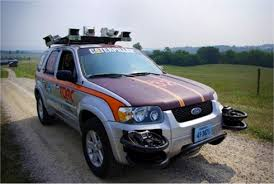
\includegraphics[width=\textwidth]{odin}
		    \end{subfigure}
		    ~
		    \begin{subfigure}[b]{0.4\textwidth}
		      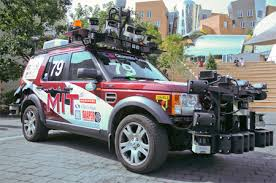
\includegraphics[width=\textwidth]{talos}
		    \end{subfigure}
		    \\~\\
		    \begin{subfigure}[b]{0.4\textwidth}
		      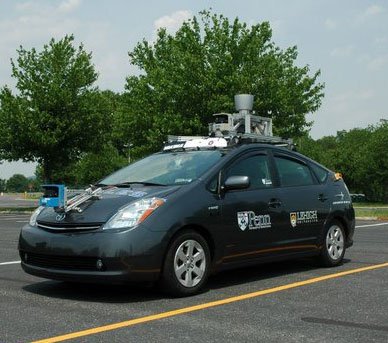
\includegraphics[width=\textwidth]{littleben}
		    \end{subfigure}
		    ~
		    \begin{subfigure}[b]{0.4\textwidth}
		      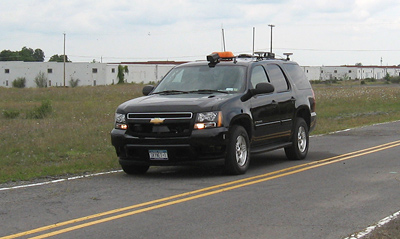
\includegraphics[width=\textwidth]{skynet}
		    \end{subfigure}

	    \end{figure}
	  \end{block}
	  }
	  \only<6>{
	  \begin{block}{Korean Autonomous Vehicle Competition (AVC)}
	    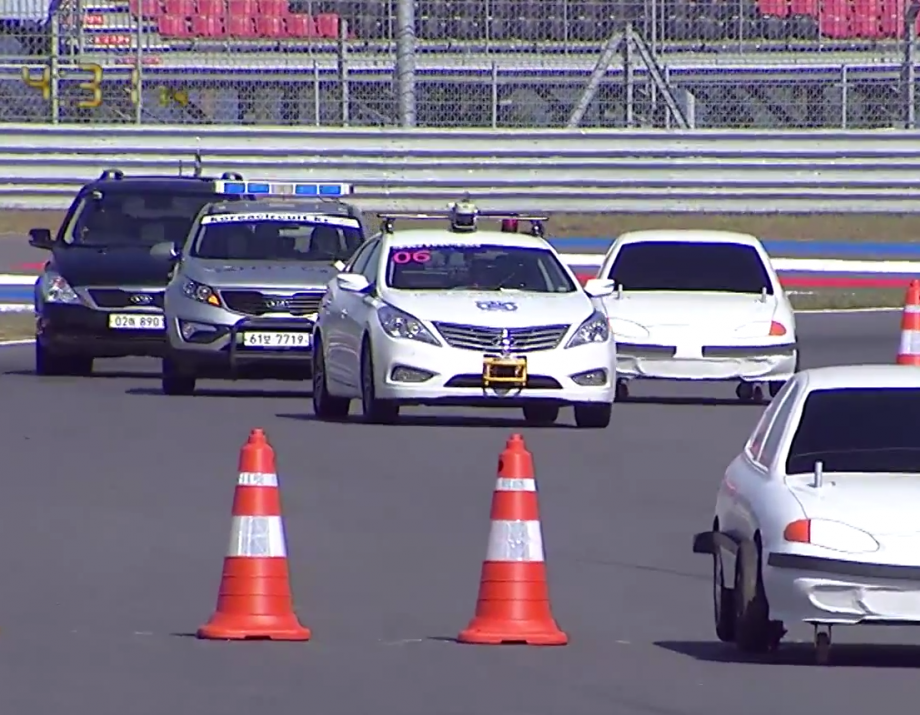
\includegraphics[width=\textwidth]{kavc}
	  \end{block}
	  }
	\end{overlayarea}
      \end{center}
    \end{columns}
    
    \note {
    \begin{itemize}
      \item From 1987 to 1995, the EC EUREKA Prometheus Project conducted research on autonomous vehicles. Among its culmination points were the twin robot vehicles VITA-2 and VaMP, driving long distances in heavy traffic.
      \item In 1996, the ARGO project modified a Lancia Thema to follow the lane marks in an unmodified highway \citep{Broggi1999}. The culmination of the project was a journey of 1,900\,km over six days on the motorways of northern Italy, with an average speed of 90 km/h. The car operated in fully automatic mode for the 94\% of its journey, with the longest automatic stretch being 55\,km. The vehicle had only two grayscale low-cost video cameras on board and used stereoscopic vision algorithms to understand its environment. 
      \item In 2004, DARPA's Grand Challenge was held in the Mojave Desert region of the United States, along a 240\,km route. This competition consisted on an autonomous vehicles race that must reach to the goal without human intervention and using just a listing of check points between the start and the finish line. None of the robot vehicles finished the route.
      \item In 2005, a second competition was held \citep{Buehler2007}. This time, five vehicles successfully completed the course:
      \begin{itemize}
      \item \emph{Stanley} \citep{thrun2006stanley}, from Standford University.
      \item \emph{Sandstorm} and \emph{H1ghlander} \citep{urmson2004high}, from the Carnegie Mellon University.
      \item \emph{Kat-5} \citep{trepagnier2006kat}, from the Gray Insurance Company.
      \item \emph{TerraMax} \citep{ozguner2004team}, from the Oshkosh Truck Corporation.
      \end{itemize}
      \item In 2007, the third driverless car competition of the DARPA Grand Challenge \citep{Buehler2009}, more known as the DARPA Urban Challenge, was held in Victorville, California. This time, six teams successfully finished the entire course:
      \begin{itemize}
      \item \emph{Boss} \citep{Urmson2008}, from the Carnegie Mellon University.
      \item \emph{Junior} \citep{montemerlo2008junior}, from Standford University.
      \item \emph{Odin} \citep{Bacha2008}, from Virginia Tech.
      \item \emph{Talos} \citep{leonard2007team}, from the Massachusetts Institute of Technology.
      \item \emph{Little Ben} \citep{bohren2008little}, from University of Pennsylvania.
      \item \emph{Skynet} \citep{miller2008team}, from Cornell University.
      \end{itemize}
      \item In 2010, 2012 and 2013, the Korean Autonomous Vehicle Competition (AVC) took place.
    \end{itemize}
    }
  \end{frame}

  \begin{frame}{Autonomous vehicles review}
    \begin{columns}[T] % the "c" option specifies center vertical alignment
      \column{.5\textwidth} % column designated by a command
      \footnotesize
      \begin{itemize}
	\item<1-> \textbf{(2010)} VIAC Challenge.
	\item<3-> \textbf{(2011)} WildCat Project.
	\item<4-> \textbf{(2011)} AutoNOMOS Group.
	\item<5-> \textbf{(2012)} Shelley.
	\item<6-> \textbf{(February 2013)} RobotCar project.
	\item<7-> \textbf{(July 2013)} BRAiVE.
	\item<8-> \textbf{(Nowadays)} Many working prototypes.
      \end{itemize}  
      \column{.5\textwidth}
      \begin{center}
	\vskip -1cm
       	\begin{overlayarea}{\textwidth}{\textheight}
	  \only<1-2>{
	  \begin{block}{VIAC Challenge}
	    \begin{itemize}
	    \item<1-> From Italy to China.
	    \item<1-> 100 day, 15,900\,km.
	    \item<2-> Four autonomous vehicles.
	    \item<2-> Limited human intervention.
	    \end{itemize}
	    \begin{center}
	      \includegraphics<1>[width=0.8\textwidth]{viacMap}
	      \includegraphics<2>[width=0.8\textwidth]{viacCars}
	    \end{center}

	  \end{block}
	  }
	  \only<3>{
	  \begin{block}{WildCat Project}
	    \begin{itemize}
	      \item Bowler Wildcat.
	      \item Oxford University.
	    \end{itemize}
	    \begin{center}\includegraphics<1->[width=\textwidth]{wildcat}\end{center}
	  \end{block}
	  }
	  \only<4>{
	  \begin{block}{AutoNOMOS Group}
	    \begin{itemize}
	      \item Spirit of Berlin.\\
	      \begin{center}\includegraphics<1->[width=0.5\textwidth]{spiritofberlin}\end{center}
	      \item MadeInGermany.\\
	      \begin{center}\includegraphics<1->[width=0.5\textwidth]{madeingermany}\end{center}
	    \end{itemize}
	  \end{block}
	  }
	  \only<5>{
	  \begin{block}{Shelley}
	    \begin{itemize}
	      \item More than 160\,km/h
	    \end{itemize}
	    \begin{center}\includegraphics<1->[width=\textwidth]{shelley}\end{center}
	  \end{block}
	  }
	  \only<6>{
	  \begin{block}{RobotCar project}
	    \begin{itemize}
	      \item Oxford University.
	      \item Switches from manual to autopilot on learned routes.
	    \end{itemize}
	    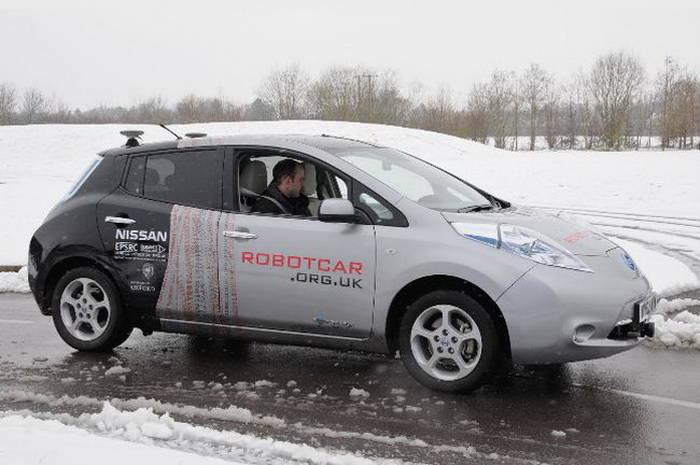
\includegraphics[width=\textwidth]{robotcar}
	  \end{block}
	  }
	  \only<7>{
	  \begin{block}{BRAiVE}
	    \begin{itemize}
	      \item Vislab.
	      \item Moved on a mixed traffic route open to public traffic.
	    \end{itemize}
	    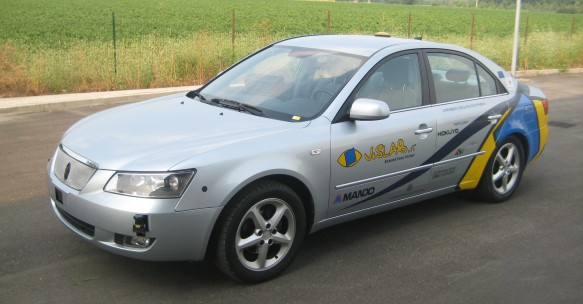
\includegraphics[width=\textwidth]{BRAiVE}
	  \end{block}
	  }
	  \only<8>{
	  \begin{block}{Many working prototypes}
	    \begin{figure}[t]
	      \centering
	      \begin{subfigure}[b]{0.2\textwidth}
		
\includegraphics[width=\textwidth]{mercedes_benz}
	      \end{subfigure}
	      ~
	      \begin{subfigure}[b]{0.2\textwidth}
		
\includegraphics[width=\textwidth]{gm}
	      \end{subfigure}
	      ~
	      \begin{subfigure}[b]{0.2\textwidth}
		
\includegraphics[width=\textwidth]{continental}
	      \end{subfigure}
	      \\~\\
	      \begin{subfigure}[b]{0.2\textwidth}
		
\includegraphics[width=\textwidth]{autoliv}
	      \end{subfigure}
	      ~
	      \begin{subfigure}[b]{0.2\textwidth}
		
\includegraphics[width=\textwidth]{bosch}
	      \end{subfigure}
	      ~
	      \begin{subfigure}[b]{0.2\textwidth}
		
\includegraphics[width=\textwidth]{nissan}
	      \end{subfigure}
	      \\~\\
	      \begin{subfigure}[b]{0.2\textwidth}
		
\includegraphics[width=\textwidth]{toyota}
	      \end{subfigure}
	      ~
	      \begin{subfigure}[b]{0.2\textwidth}
		
\includegraphics[width=\textwidth]{audi}
	      \end{subfigure}
	      ~
	      \begin{subfigure}[b]{0.2\textwidth}
		
\includegraphics[width=\textwidth]{vislab_logo}
	      \end{subfigure}
	      \\~\\
	      \begin{subfigure}[b]{0.2\textwidth}
		
\includegraphics[width=\textwidth]{oxforduni_logo}
	      \end{subfigure}
	      ~
	      \begin{subfigure}[b]{0.2\textwidth}
		
\includegraphics[width=\textwidth]{google}
	      \end{subfigure}
	    \end{figure}
	  \end{block}
	  }
	\end{overlayarea}
      \end{center}
    \end{columns}
    
    \note {
    \begin{itemize}
      \item In 2010, inside the VIAC Challenge, four autonomous vehicles drove from Italy to China on a 100-day 15,900\,km trip with only limited human intervention (in traffic jams and when passing toll stations). At the time, this was the longest-ever journey conducted by an unmanned vehicle \citep{Broggi2010VIAC}.
      \item In 2011, under the Oxford University's WildCat Project, a Bowler Wildcat based prototype is capable of autonomous operation using a flexible and diverse sensor suite.
      \item In 2011, the Freie Universität Berlin, Led by the AutoNOMOS group, developed two autonomous cars - \emph{Spirit of Berlin} \citep{berlin2007spirit} and \emph{MadeInGermany} \citep{gohring2013semi} - to drive in the innercity traffic of Berlin in Germany. They were able to handle intercity traffic, traffic lights and roundabouts between the International Congress Centrum and the Brandenburg Gate.
      \item In 2012, Stanford's Dynamic Design Lab, in collaboration with the Volkswagen Electronics Research Lab, produced Shelley, an Audi TTS designed for high speed (greater than 160\,km/h) on a racetrack course.
      \item In February 2013, Oxford University unveiled the RobotCar UK project, an inexpensive autonomous car capable of quickly switching from manual driving to autopilot on learned routes.
      \item In July 2013, Vislab worldpremiered BRAiVE, a vehicle that moved autonomously on a mixed traffic route open to public traffic \citep{grisleri2010braive}.
      \item Currently, many major companies and research organizations have developed working prototype autonomous vehicles, including Mercedes-Benz, General Motors, Continental Automotive Systems, Autoliv Inc., Bosch, Nissan, Toyota, Audi, Vislab (University of Parma), Oxford University and Google.
    \end{itemize}
    }
  \end{frame}
  
  \begin{frame}{Obstacle detection}
    We can divide object tracking methods into two subcategories:
    \begin{itemize}
      \item \emph{2.5D Solutions:} Different approaches:
      \begin{itemize}
	\item \emph{Use of the 3D point as feature.} \cite{franke20056d}
	\item \emph{Dynamic stixels.} \cite{badino2009stixel, pfeiffer2011towards, pfeiffer2013exploiting, benenson2011stixels, benenson2012pedestrian, benenson2012fast}
	\item \emph{Tracked image features.} \cite{barth2009estimating}
	\item \emph{Sensor fusion.} \cite{wu2009collision}
	\item \emph{Occupancy grids.} \cite{danescu2012particle}
      \end{itemize} 
      \item \emph{3D Solutions}
      \begin{itemize}
	\item \emph{Octree connected cubes.} \cite{broggi2013}
	\item \emph{Adjacent stacks of cells} \cite{Moravec96robotspatial}
      \end{itemize}
    \end{itemize}
    
    \note{
    Based on how much information they use, we can divide object tracking methods into two subcategories:
    \begin{itemize}
      \item \emph{2.5D Solutions:} They do not make use of the complete information provided by 3D points. Instead of that, they tend to use elevation maps composed of uniform size cells. Each cell just stores occupancy and height information. This is the kind of methods that, as described before, usually consider obstacles as being in contact with a flat ground.
      In these methods, tracking is performed before the complete reconstruction is done, in an intermediate point based on an specific feature. Depending on the feature used, we distinguishing different approaches:
      \begin{itemize}
	\item \emph{Use of the 3D point as feature.} An example of this is the so called 6D vision \citep{franke20056d}, in which the 3D stereo vision extracted information is combined with an efficient implementation of an optical flow in the image space based on a \ac{GPU}. Relevant points are tracked using a Kalman filter.
	\item \emph{Dynamic stixels.} This approach has been longer discussed in section \ref{ch:chapter00_02_04}.
	\item \emph{Tracked image features.} An example is the work by \cite{barth2009estimating}. There, obstacles are represented as a rigid 3D point set which are tracked in terms of feature displacements and depth measurements.
	\item \emph{Sensor fusion.} \cite{wu2009collision} reconstruct the objects as cuboids from a stereo point cloud. In this process, position and speed values are improved to a very accurate value by the use of a radar along with stereo.
	\item \emph{Occupancy grids.} This is a very popular choice for tracking. An occupancy grid is a probabilistic map of the driving environment, which encodes the past and present knowledge from sensor data, and which can be updated dynamically when new information is available. These occupancy grids can be cartesian, with rectangular cells, polar, or even a relation between columns in an image and the disparity. An example of this is the method by \cite{danescu2012particle}, which has inspired part of the work described in chapter \ref{ch:chapter05}.
	Another advantage of the model based on an occupancy grid is that it makes easier a collaborative update of the grid, which allows the usage of data from several sensors and observers. Another simple example of occupancy grid is that described in chapter \ref{ch:chapter07}.
      \end{itemize} 
      \item \emph{3D Solutions:} Usually based on complex grid maps that use complete 3D information. Again, depending on how this grid is represented, we find 
      \begin{itemize}
	\item \emph{Octree connected cubes.} An example is the work by \cite{wurm2010octomap} or \cite{broggi2013}.
	\item \emph{Adjacent stacks of cells}, as described in \cite{Moravec96robotspatial} 
      \end{itemize}
    \end{itemize}
    }
  \end{frame}

  \begin{frame}{Path planning}
    \begin{itemize}
      \item Classical methods \citep{hwang1992gross}
      \item Heuristic methods \citep{masehian2007classic}
      \item SVM based methods
      \begin{itemize}
       \item Global
	 \begin{itemize}
	  \item \cite{miura2006support}
	  \item \cite{yang2012safe}
	 \end{itemize}
       \item Local
	\begin{itemize}
	  \item \cite{sarkar2008mobile}
	  \item \cite{tennety2009support}
	  \item \cite{qingyang2012local}
	\end{itemize}
      \end{itemize}
    \end{itemize}
    
    \note{
      About classical methods, in general they can be considered as variations of some general approaches: Roadmap, Cell Decomposition, Potential Fields and Mathematical Programming. These methods are not mutually exclusive; in fact, a lot of approaches use combinations of them. A review of some classical methods can be checked out in \cite{hwang1992gross}.
 
      About heuristic methods, these are the answer given by researchers to the limitations of the classic methods. The most representative methods inside this classification are Probabilistic Roadmaps (PRM) \citep{kavraki1996probabilistic}, Rapidly Exploring Random Trees (RRT) \citep{lavalle2000rapidly}, Level set \citep{sethian1999level}, Linguistic Geometry (LG) \citep{stilman1993network}, Simulated Annealing (SA) \citep{zhu2006robot}, Artificial Neural Network (ANN) \citep{hossain2012real}, Genetic Algorithms (GA) \citep{zhang2007evolutionary}, Particle Swarm Optimization (PSO) \citep{chen2006smooth}, Ant Colony (ACO) \citep{mou2008modified} and its variants, like the RNA algorithm described in \cite{zhu2011new}, Stigmergy \citep{cazangi2006evolutionary}, Wavelet Theory \citep{doh2005systematic}, Fuzzy Logic (FL) \citep{kladis2011energy} and Tabu Search (TS) \citep{nguyen2012multi}. For more information, the review in \cite{masehian2007classic} can be checked.
      
      Global:
      In the work presented by \cite{miura2006support}, navigation is planned in environments in which the obstacles are known. Obstacles are randomly labeled into two classes: positive or negative. Using these two classes, a \ac{SVM} is trained and the decision boundary is used as a path. To increase the efficiency, a set of fake obstacles (guide samples) is generated at both sides of the current and goal position, as well as in parallel to the line that joins both points (nominal line), with the objective of helping the \ac{SVM} to find a feasible path.
      \cite{yang2012safe}. In their work, a preprocessing step is used in which the Voronoi Diagram is generated using the obstacles in the map. That diagram is used to select the best path between the starting point of the robot and the goal. The path obtained using Voronoi is not smooth, so the \ac{SVM} is used to make this path smoother. The \ac{SVM} is trained using a dataset in which the sites that generated the Voronoi edges are classified as positive or negative depending on their position (left / right) regarding to the previously obtained path. The decision boundary of this \ac{SVM} will be the final path used.
      
      Local:
      In \cite{sarkar2008mobile, tennety2009support}, authors divide the whole set of objects in the map into two classes and the \ac{SVM} is used to determine the maximum margin hyperplane between the data sets belonging to the two classes. Data is assigned to one or another class depending on whether the points are on the left or on the right side of the robot. Once the initial labels are assigned, further classification is done using the k-nearest neighbor algorithm, with k=1.
      \cite{qingyang2012local}, that uses a path subdivision method and a \ac{SVM}. They use topological maps of local environments which are extracted with little expanded nodes. Next, candidate routes are optimized using the Support Vector Machine, where the candidate routes boundary points are defined as positive and negative samples. They also extend the original \ac{SVM} \citep{cortes1995support} in order to satisfy extra constraints such as vehicle position and heading.
    }
  \end{frame}
  
    \begin{frame}{Local planning}
    \begin{itemize}
      \item \cite{werling2010optimal}
      \item \cite{thrun2006stanley}
      \item \cite{chu2012local}
    \end{itemize}
     
    \note{
      \begin{itemize}
	\item In \cite{werling2010optimal}, long term objectives are performed, like speed keeping, merging, following, stopping. This is done through optimal control strategies within the Fren\'et frame of the street.
	\item In \cite{thrun2006stanley}, lateral offset is defined as the perpendicular to an established base trajectory. This allows the vehicle driving along the road parallel to this trajectory. In order to select the optimal path, the cost function penalizes passing over obstacles and the distance respect to the center of the current road.
	\item In \cite{chu2012local}, also a set of candidate paths are generated, with endpoints in fixed positions at different offsets respect to the base frame, but they do not set this base frame in the center of the road, since it could be dangerous when computing the costs at certain scenarios. Instead of that, they use a security cost for each candidate path. Security of the path is computed by blurring the binary data of the obstacles. They also have into account certain criteria, as the smoothness cost or the path consistency between iterations.
      \end{itemize}
    }
  \end{frame}
  
  \subsection{Testing platform}
  \begin{frame}{Testing platform}
    These algorithms are intended to be used in Verdino.
    \begin{itemize}
     \item<1-> Prototype developed by GRULL, Universidad de La Laguna.
     \item<2-> It will transport people around a bioclimatic urbanization in the ITER facilities.
     \item<3-> A golf cart has been modified to be used as an unmanned vehicle.
    \end{itemize}

    \begin{center}
      \includegraphics<1-1>[height=.3\columnwidth]{verdino}
      \includegraphics<2-2>[height=.3\columnwidth]{iter}
      \includegraphics<3-4>[height=.3\columnwidth]{NV_TXT2}
      \includegraphics<4-4>[height=.3\columnwidth]{verdino}
    \end{center}
  \end{frame}
  
  \begin{frame}{Actuators}
    \begin{columns}[c] % the "c" option specifies center vertical alignment
      \column{.5\textwidth} % column designated by a command
      \begin{itemize}
	\item<1-> Steering system.      
	\item<2-> Braking system.
	\item<3-> Speed system.
	\item<4-> Safety switch.
      \end{itemize}  
      \column{.5\textwidth}
      \begin{center}
	\includegraphics<1-1>[width=\textwidth]{steering}
	\includegraphics<2-2>[width=\textwidth]{braking}
	\includegraphics<3-3>[width=\textwidth]{speedControl}
	\includegraphics<4-4>[width=\textwidth]{panicbutton}
      \end{center}
    \end{columns}
    
    \note {
    \begin{itemize}
      \item Steering system: we tied the original steering to a DC motor controlled by a PID.
      \item Braking system: Controlled through a pneumatic system, composed by a cylinder, a commutation valve, two flow controllers and an air compressor. The pneumatic cylinder acts over the brake cables, that make pressure over the brake drums. A compressor gives the air pressure needed for this process.
      \item Speed system: A microcontroller generates three different signals, that simulate the original devices installed in the vehicle. These correspond to a switch relay, which turns on the motor when the user pushes the acceleration pedal; the sense of speed (forward or backward); and the desired voltage
      \item Safety switch: Allows changing between automatic and manual behavior. When switched off, the vehicle behaves as it was before the modifications.
    \end{itemize}
    }
  \end{frame}

  \begin{frame}{Sensors}
    \begin{columns}[c] % the "c" option specifies center vertical alignment
      \column{.5\textwidth} % column designated by a command
      \begin{itemize}
	\item<1-> Localization sensors.      
	\begin{itemize}
	  \item<3-> Odometry.      
	  \item<4-> IMU.
	  \item<5-> Differential GPS.
	\end{itemize}  
	\item<2-> Navigation sensors.	
	\begin{itemize}
	  \item<6-> LIDAR.      
	  \item<7-> IR cameras.
	  \item<8-> Visible cameras.
	\end{itemize}
      \end{itemize}  
      \column{.5\textwidth}
      \begin{center}
	\includegraphics<3-3>[width=\textwidth]{odometry}
	\includegraphics<4-4>[width=\textwidth]{imu}
	\includegraphics<5-5>[width=\textwidth]{dgps}
	\includegraphics<6-6>[width=\textwidth]{lidar}
	\includegraphics<7-7>[width=\textwidth]{ircameras}
	\includegraphics<8-8>[width=\textwidth]{visiblecamera}
      \end{center}
    \end{columns}
    
    \note {
    \begin{itemize}
      \item \emph{Odometry}: This system measures the independent movement of the two rear wheels, which are attached to an optical encoder. This allows computing the position, orientation and speed of the prototype incrementally.
      \item \emph{\acf{IMU}}: It is comprised by 9 sensors (3 accelerometers, 3 gyroscopes and 3 magnetometers), which are fused in real time in order to get the three-dimensional orientation of the vehicle. The model of the sensor is a \emph{Xsens Mti}.
      \item \emph{\acf{DGPS}}: Allows positioning the vehicle with centimetric accuracy. It is composed by two different devices, the reference station, which is fixed in a known place, and the rover station, which is installed on the vehicle. The model used is a \emph{JAVAD GNSS Triumph-1}, which has an horizontal precision below 1\,cm and a vertical precision around 1.5\,cm using \ac{DGPS}, at a frequency of $5\,Hz$.
      \item \emph{\acf{LIDAR}}: These are used also for localization purposes. Each of those sensors is able to detect the objects in the way of the vehicle, at the plane in which the sensor is mounted. The advantages of these sensors are that they have a high speed and precision. However, they are just able to detect obstacles that crosses the plane defined by the sensor. Because of this, we have equipped the vehicle with 5 \acp{LIDAR}. Two of them are located at the same plane in the front corners of the vehicle, at a height of 50\,cm. Each of these covers an angle of 270\textdegree. Another is located in the front side of the vehicle, at a height of 20\,cm, slightly tilted upwards, in order to detect the small obstacles or non traversable areas. Another is in the top of the vehicle, also in the front side of the vehicle, tilted to the ground and covering the blind areas left by the other sensors. Finally, the last sensor is situated in the back side of the vehicle, and it is used for backwards maneuvers. The used sensors are of the model \emph{SICK LMS 100} and \emph{SICK LMS 111}, allowing a maximal detection distance of 20\,m, a precision of 10-35\,mm, a maximal angular resolution of 0.25\textdegree and a maximal rate of $50\,Hz$.
      \item \emph{IR cameras}: Infrared cameras are used to detect pedestrians or animals based on their temperature. We have a pair of them installed on a Pan-Tilt system attached to the top front side of the vehicle. The model used is a \emph{MobiR\textregistered~M3}, which is able to detect objects in the range $8\sim14\mu m$, at a resolution of $160 \times 120\,px$.
      \item \emph{Visible cameras}: A set of three cameras is also installed in a pan-tilt structure. These are used for the detection and tracking of the objects, which is one of the goals of this thesis. Also, they are currently being used for the detection of the borders of the road. The model of the cameras is a \emph{GoPro\textregistered Hero 3 silver edition}, with a $1920 \times 1080 \, px$ maximal video resolution and a 170\textdegree field of view at a maximal rate of 60\,fps.
    \end{itemize}
    }
  \end{frame}
  
  \begin{frame}{Control}
    \begin{columns}[c] % the "c" option specifies center vertical alignment
      \column{.5\textwidth} % column designated by a command
      \begin{itemize}
	\item<1-> Onboard computer.   
	\begin{itemize}
	  \item<2-> i7-3770K.      
	  \item<2-> 16 Gb RAM DDR3.
	  \item<2-> SSD Storage.
	\end{itemize}	
	\item<3-> Low-level control.
      \end{itemize}  
      \column{.5\textwidth}
      \begin{center}
	\includegraphics<1->[width=\textwidth]{onboard}
      \end{center}
    \end{columns}
    
    \note {
    The vehicle is controlled, at high level, by an on board computer equipped with an \emph{i7-3770K} processor, 16\,Gb of \emph{RAM DDR-3} memory and a \emph{SSD} storage. At low level, a set of own developed electronic devices receive commands from the computer and transform them into the right signal, understandable by the actuators described before.
    }
  \end{frame}
  
\section{Obstacle Detection}
% %%
%%  chapter01.tex - Obstacle Detection and Planning for Autonomous Vehicles based on Computer Vision Techniques
%%
%%  Copyright 2014 Néstor Morales <nestor@isaatc.ull.es>
%%
%%  This work is licensed under a Creative Commons Attribution 4.0 International License.
%%

\graphicspath{{./images/chapter01/bmps/}{./images/chapter01/vects/}{./images/chapter01/}}

\chapter{Problem Statement and Previous Work}\label{ch:chapter01}

\section{Problem Statement}\label{ch:chapter01_01}

Computer Vision environment understanding targeted at enabling autonomous operation of a robotic platform has been widely studied over the years, leading to the creation of some prototype vehicles \cite{Maurer1996,Pomerleau1996,Broggi1999} which demonstrated that negotiating moderately complex and dynamic situations in real time was possible, albeit challenging. However, it was only with the development effort driven by the DARPA Challenges \cite{Buehler2007, Buehler2009} that the technology required to provide reliable operation both in off-road and urban scenarios proved to be within reach.
The vehicles that successfully took part to this series of events had to integrate planning and actuation capabilities with a sensing suite capable of coping with harsh environments, heavy traffic and wide temperature ranges, while keeping functional over extended amounts of time. Most competitors relied on high-end active sensors \cite{Urmson2008, Montemerlo2008, Bacha2008, Kammel2008}, with some notable exceptions \cite{Broggi2006, Broggi2010}. 

As we discover when looking up to the available literature (See next section, \ref{ch:chapter01_02}), there are many methods for the detection and tracking of obstacles in complex environments, like this for which Verdino is intended to be working. In this sense, a very first approach is that inspired on the work by \cite{primdahl2005change},  \cite{diego2011video} or \cite{vallespi2012prior} was developed. This is based on the fact that, in an image, a high percentage of the scene represented usually corresponds to static objects. Based on that, it looks quite straightforward to think that, having an image representing an area without obstacles, it is possible to detect the obstacles in an scene by just comparing it with an image being taken in real time. For that, we obtained a dataset with geo-referenced images from a closed urbanization taken at different times of the day. A description of this database, as well as of the algorithm pipeline used for the comparison between images pairs can be found at section \todo{ \ref{XXX} }.

However, such approach suffers from several drawbacks. First, as we just use one image per frame, we are no able to know the exact position of the obstacle in the real world \comment{(Anyway, we think that the output of the algorithm is a good starting point for a classification method)}. Also, the quality of detection is highly tied to the size of the image database, so in big areas we need a huge dataset, with the related space and throughput problems associated to that. If we consider changes due to weather or light conditions, this dataset grows exponentially. Finally, we don't know the direction where an obstacle is going to. These are challenging problems that have been solved using different approaches, until we reached a final solution, described in section \todo { \ref{XXX} }.

To solve that, we first developed a method that tries to isolate just the tracking problem with the use of static monocular cameras. Instead of registering pairs of images, we segment the image with the use of foreground extraction techniques, distinguishing between background and foreground. Using the silhouette of the objects in the foreground (which are mainly non-rigid objects, like pedestrians or animals), we apply a non-rigid point set registration algorithm in order to track the different parts of the body of the obstacles separately. This method, inspired in works like those by \cite{starck2007surface}, or \cite{letouzey2011scene}, can be also used for the completion of the global map of the vehicle, or even for tasks more related to \acf{HMI}. This approach is extensively described in section \todo{ \ref{XXX}}.

However, this method still makes use of a very rudimentary method for the localization of the obstacles (See section \todo{ \ref{XXX-subsection_localization}}), and it is limited to static cameras. For the application proposed, we need the cameras installed on the top of the moving prototype, so we can not use foreground segmentation methods anymore for the detection of the objects in the road. A simple solution for that is stop using monocular vision, and start using stereo vision. In the last years, a high number of advanced algorithms has become viable for autonomous driving applications. The problem is that performing a quantitative and meaningful comparison of their performance level, however, is not an easy task, mainly because of the difficulty of producing ground truth information. Older datasets are small, and either synthetic or taken in controlled environments (\cite{Scharstein2002}), thus effectively limiting their usefulness as indicators of the actual algorithms ability to cope with outdoor scenarios. Due to that, it is needed to compare the performance level of some state-of-the-art stereovision-based 3D mapping algorithms in automotive scenarios. This evaluation methodology and the associated results is shown in section \todo{ \ref{XXX}}. \comment{PREGUNTAR A LA GENTE DEL VISLAB SI ESTA DE ACUERDO CON QUE USE ESTO EN LA TESIS, POR SI LAS MOSCAS}.

\comment{Este párrafo y la sección asociada dependerá de lo que consiga sacar más adelante.}\notsure{
Apart from the full-dense 3D reconstruction methods, we also explore the possibility of using a simpler (and faster) reconstruction based on Stixels, like that described by \cite{badino2009stixel}. In particular, we decided to use the implementation by \cite{benenson2012pedestrian}, due to its fast response (about 100 frames per second). The method, described in section \todo{\ref{XXX}}, compares the stixels obtained between frames and tracks the obstacles along the time. This solves all the problems we had: we can use moving cameras, we can locate the obstacles in the map, and also we are able to know the path followed by them.}

Another approach, which makes use of the dense stereo reconstruction algorithms for which we did the evaluation described above, is inspired in the work by \cite{danescu2012particle}, but also from the voxelized world described in \cite{broggi2013}. The key idea is to simplify the 3d reconstructed world into a grid of voxels, each of these representing a certain volume in the world. In this voxelized world, for each voxel above a given occupancy probability threshold, a set of particles part of a particle filter is assigned. Each particle will have a double function: the first, denoting hypotheses (as in the classical particle filter methods); the second, to be used as segmentation criteria in the segmentation of the world into different obstacles. In this way, we consider that two contiguous voxels belong to different obstacles if their obtained direction and sense diverges. A more detailed explanation of the method is found in \todo{\ref{XXX}}.

At this point, we have an acceptable reconstruction of the surroundings of the vehicle, which includes the localization and tracking of the obstacles in the neighborhood of the cart. But the reconstruction of the environment is not the only challenge that an autonomous vehicle has to deal with. Once that a vehicle has an idea of where it is, and where it wants to go, it also needs to know the best way to reach there and, more important, how to avoid the harmful elements it has previously detected using the methods described. This allows a safe trip, both for the pedestrians, cars, etc. in the road, and for the vehicle itself.
As said, Verdino is intended to travel in pedestrian areas where most of the obstacles are pedestrians, so its behavior must be mainly reactive in order to give priority to the safety of paths against the efficiency of the route. Also, there is not a clear traveling path, like a road. Instead of that, the vehicle will be moving around an unstructured area, so there is not something like a \acf{RNDF} that allows a fast calculation of the paths that the car will use to reach a certain point. Because of that, we must consider two different planning levels:
\begin{itemize}
 \item \textbf{Global Planning:}
 As it is not possible to determine a global trajectory based on a \acs{RNDF}, we must use a method able to deal with changing environments for the calculation of a fast and safe path. The idea is that, having a map of the static obstacles in the environment and with the vehicle properly localized on it \cite{Perea2013mcl}, it will generate a path that will allow reaching this destination as fast as possible. This task, which can be solved easily in static environments using graphs or other similar optimization methods, becomes a little bit more challenging in environments like, for example, a parking lot, in which cars are parking and driving off continuously.
 In section \todo{ \ref{XXX} }, the way in which we solved this problem is described. It is based on the border between classes, which is obtained after training a \acf{MSVM} (See Appendix \todo {\ref{XXX}} for more information), considering each single obstacle as a separate class. Instead of using this border for classification purposes, as it is usual, we take advantage of the fact that it will be the safest and smoother distance to the obstacles. Taking this into account, it makes sense to apply this separation line as our path. Also, the use of a different class for each obstacle allows ensuring that the path is safe enough, even in complicate scenarios, like in pedestrian areas.
 
 \item \textbf{Local Planning:}
 In a lower level, we also need a way to make the vehicle know how to follow the generated path. This problem requires a system able to, several times per second, calculate the best steering angle and speed in order to follow the global plan while avoiding the surrounding obstacles. The method, which is inspired in the work of \cite{chu2012local}, receives as input the current position of the vehicle in the map, its orientation, speed and the steering angle. Also, we provide it with the global plan obtained in the upper level. Finally, a map of the dynamic obstacles in the surrounds of the cart is computed and passed to the algorithm.
 
 This dynamic map can be filled with the information provided by sensors like \acp{LIDAR}, among other sensors. But it can can also be computed with the information extracted from cameras, and this is the connection point with the work described in the first part of this Thesis. The detected obstacles are included in the map, so the vehicle is able to avoid them using the calculated steering angle and speed.
 
 The way in which both this map and the speed/steering angle commands is obtained is described in section \ref{XXX}.
\end{itemize}
 
 The whole pipeline of the application developed for this thesis is shown at figure \ref{fig:cp01_pipeline}. 
 
\begin{figure}[thb]\label{fig:cp01_pipeline}
  \centering
  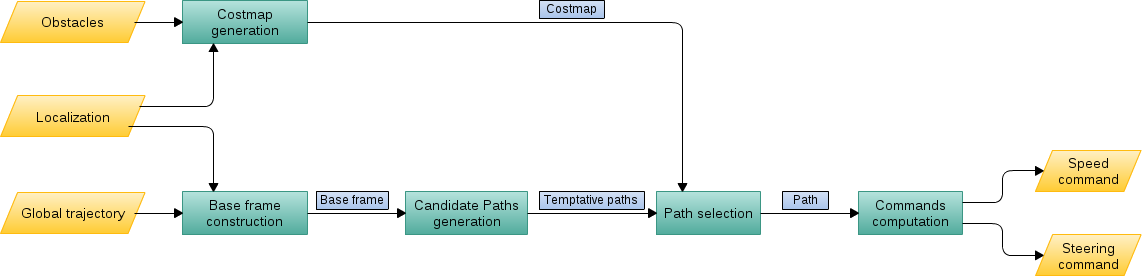
\includegraphics{pipeline}
  \caption{Pipeline of the modules described in this Thesis.}
\end{figure}

From the images captured in real-time, obstacles are located and passed to the module in charge of the generation of the dynamic costmap. At the same time, the static map is used for the generation of a feasible trajectory. Using the current position and vehicle status, the local planner tries to compute the proper commands in order to follow the global plan while trying to avoid the obstacles included in the dynamic costmap.

\section{Previous Work}\label{ch:chapter01_02}

Research on autonomous vehicles is a task being developed for a long time and for which a big effort has been carried on. A proof of that is the extensive literature existing about that topic, in special since the first of the DARPA Challenges (\cite{Buehler2007, Buehler2009}). Since then, the literature related to the topic has increased. Also, the interest on the use of Computer Vision in autonomous vehicles is growing, due to the possibilities that images offer when compared to other sensors, like \acp{LIDAR}.
In 1996, the ARGO project... \todo{Continuar desde aquí, una vez tenga una especie de historia de los vehiculos autonomos, en la intro.}
\todo{TerraMax, VIAC, Braive, Annieway y cualquier otro que pille por el camino.}
As depicted from section \ref{ch:chapter01_01}, the topics described in this thesis are quite diverse, so it is fair to review the state-of-the art of each of these topics separately.

\subsection{Change detection for obstacle localization in images}\label{ch:chapter01_02_01}

\todo{blah blah blah blah blah blah blah blah blah blah blah blah blah blah blah blah blah blah blah blah blah blah blah blah blah blah blah blah blah blah blah blah blah blah blah blah blah blah blah blah blah blah blah blah blah blah blah blah blah blah blah blah blah blah blah blah blah blah blah blah blah blah blah blah blah blah blah blah blah blah blah blah blah blah blah blah blah blah blah blah blah blah blah blah blah blah blah blah blah blah blah blah blah blah blah blah blah blah blah blah blah blah blah blah blah blah blah blah blah blah blah blah blah blah blah blah blah blah blah blah blah blah blah blah blah blah blah blah blah blah blah blah blah blah blah blah blah blah blah blah blah blah blah blah blah blah blah blah blah blah blah blah blah blah blah blah blah blah blah blah blah blah blah blah blah blah blah blah }

\subsection{Non-rigid point set registration for obstacle tracking}\label{ch:chapter01_02_02}

\todo{blah blah blah blah blah blah blah blah blah blah blah blah blah blah blah blah blah blah blah blah blah blah blah blah blah blah blah blah blah blah blah blah blah blah blah blah blah blah blah blah blah blah blah blah blah blah blah blah blah blah blah blah blah blah blah blah blah blah blah blah blah blah blah blah blah blah blah blah blah blah blah blah blah blah blah blah blah blah blah blah blah blah blah blah blah blah blah blah blah blah blah blah blah blah blah blah blah blah blah blah blah blah blah blah blah blah blah blah blah blah blah blah blah blah blah blah blah blah blah blah blah blah blah blah blah blah blah blah blah blah blah blah blah blah blah blah blah blah blah blah blah blah blah blah blah blah blah blah blah blah blah blah blah blah blah blah blah blah blah blah blah blah blah blah blah blah blah blah }

\subsection{Evaluation of stereo 3D reconstruction algorithms}\label{ch:chapter01_02_03}

\todo{blah blah blah blah blah blah blah blah blah blah blah blah blah blah blah blah blah blah blah blah blah blah blah blah blah blah blah blah blah blah blah blah blah blah blah blah blah blah blah blah blah blah blah blah blah blah blah blah blah blah blah blah blah blah blah blah blah blah blah blah blah blah blah blah blah blah blah blah blah blah blah blah blah blah blah blah blah blah blah blah blah blah blah blah blah blah blah blah blah blah blah blah blah blah blah blah blah blah blah blah blah blah blah blah blah blah blah blah blah blah blah blah blah blah blah blah blah blah blah blah blah blah blah blah blah blah blah blah blah blah blah blah blah blah blah blah blah blah blah blah blah blah blah blah blah blah blah blah blah blah blah blah blah blah blah blah blah blah blah blah blah blah blah blah blah blah blah blah }

\subsection{Stixel World}\label{ch:chapter01_02_04}

\todo{blah blah blah blah blah blah blah blah blah blah blah blah blah blah blah blah blah blah blah blah blah blah blah blah blah blah blah blah blah blah blah blah blah blah blah blah blah blah blah blah blah blah blah blah blah blah blah blah blah blah blah blah blah blah blah blah blah blah blah blah blah blah blah blah blah blah blah blah blah blah blah blah blah blah blah blah blah blah blah blah blah blah blah blah blah blah blah blah blah blah blah blah blah blah blah blah blah blah blah blah blah blah blah blah blah blah blah blah blah blah blah blah blah blah blah blah blah blah blah blah blah blah blah blah blah blah blah blah blah blah blah blah blah blah blah blah blah blah blah blah blah blah blah blah blah blah blah blah blah blah blah blah blah blah blah blah blah blah blah blah blah blah blah blah blah blah blah blah }

\subsection{3D object tracking}\label{ch:chapter01_02_05}

By processing the data captured by sensors, it is desired to obtain the position, speed and size of an obstacle. However, usually sensors don't provide this information, so we need to process the information over time and do the tracking of detected obstacles. Many approaches that try to solve this problem, like \cite{danescu2012particle}, assume that obstacles have an standard geometry, and they are modeled as cuboids with associated position, size and speed vectors. This assumption is mostly correct in environments like highways, country roads, and certain urban scenarios, in which almost all the obstacles are cars, trucks or buses which can be simplified as cuboids. Also, these approaches tend to consider a flat ground.
However, this assumption cannot always done, as happens in pedestrian areas, intersections, off-road... In this case, we need to deal with specific shapes, sometimes with concave surfaces. The problem with this kind of obstacles is that methods that assume cuboid-shaped objects tend to wrap the obstacles with a convex shape, which causes an overestimation of their volume (\cite{broggi2013}). Another problem are those objects that are not laying on the ground, as happens with hanged traffic lights, tree crowns, lamps, etc. Usually, they are integrated into an occupancy grid as if they were touching the ground. About the ground plane assumption, in cases like that of an off-road scenario, it is important to estimate the real slope of the road in order to get good results.
Based on how much information they use, we can divide object tracking methods into two subcategories:
\begin{itemize}
 \item \emph{2.5D Solutions:} They do not make use of the complete information provided by 3D points. Instead of that, they tend to use elevation maps composed of uniform size cells. Each cell just stores occupancy and height information. This is the kind of methods that, as described before, usually consider obstacles as being in contact with a flat ground.
 In these methods, tracking is done before the complete reconstruction is done, in an intermediate point based on an specific feature. Based on this intermediate feature, we can distinguishing different kind of approaches:
  \begin{enumerate}
   \item \emph{Use of the 3D point as feature.} An example of this is the so called 6D vision (\cite{franke20056d}), in which the 3D stereo vision extracted information is combined with an efficient implementation of an optical flow in the image space based on a \acf{GPU}. Relevant points are tracked using a Kalman filter.
   \item \emph{Dynamic stixels.} \todo{This approach has been longer discussed in section \ref{ch:chapter01_02_04}.}\comment{Cambiar en caso de que al final no meta los stixels}
   \item \emph{Tracked image features.} As example, check the work by \cite{barth2009estimating}. In this work, obstacles are represented as a rigid 3D point set which are tracked in terms of feature displacements and depth measurements.
   \item \emph{Sensor fusion.} \cite{wu2009collision} reconstruct the objects as cuboids from a stereo point cloud. In this process, position and speed values are improved to a very accurate value by the use of a radar along with stereo.
   \item \emph{Occupancy grids.} This is a very popular choice for tracking. An occupancy grid is a probabilistic map of the driving environment, which encodes the past and present knowledge from sensor data, and which can be updated dynamically when new information is available. These occupancy grids can be cartesian, with rectangular cells, polar, or even a relation between columns in an image an the disparity. An example of this is the method by \cite{danescu2012particle}, which has inspired part of the work described in section \todo { \ref{XXX}}.
   Another advantage of the model based on an occupancy grid is that it makes easier a collaborative update of the grid, which allows the usage of data from several sensors and observers.
  \end{enumerate} 
 \item \emph{3D Solutions:} Usually based on complex grid maps that use complete 3D information. Again, depending on how this grid is represented, we find 
 \begin{enumerate}
   \item \emph{Octree connected cubes.} An example is the work by \cite{wurm2010octomap} or \cite{broggi2013}.
   \item \emph{Adjacent stacks of cells}, as described in \cite{Moravec96robotspatial} 
 \end{enumerate}
\end{itemize}

\subsection{Global planning}\label{ch:chapter01_02_06}

Muchos estudios se han realizado en torno al problema de generacion de rutas globales. Aunque fue inicialmente propuesta para aplicaciones en robotica, ultimamente se ha usado con exito en aplicaciones de automocion.

Podemos dividir los algoritmos de planificacion en... (El resto esta en la libreta, en la parte de estado del arte de planificacion local)


==============================================================
Lo que pongo a continuacion va para la intro de global planning
Los algoritmos de planificacion pueden ser divididos en locales y globales:
Globales:
  La ruta global y los estados del vehiculo quedan determinados por la info proporcionada por un mapa digital y un sistema de localizacion
Locales:
  La ruta local puede ser generada entonces en la etapa de planificacion basada en la ruta global y la info del entorno del vehiculo obtenida por los sensores
  El paper se basa en local path planning que proporciona capacidades de evitacion de obstaculos a un vehiculo autonomo que sigue una ruta global predefinida


\subsection{Local planning}\label{ch:chapter01_02_03}

Con una ruta global calculada y el conocimiento del entorno del vehículo, hace falta enviar al vehículo una serie de comandos que le indiquen cómo seguirla.

En la literatura, muchos métodos se basan en la búsqueda de trayectorias que hagan de intermediarias entre esta ruta global y la ruta local.

Muchos de estos métodos de generación trayectorias se basan en un esquema de optimización discreta (refs. 6, 17-19 coreanos)

Estos métodos calculan un cjto finito de trayectorias basadas en un modelo parametrico, habitualmente funciones polinomiales de un orden determinado. El problema de esto es que a pesar de q el espacio de sol. se reduce y permite una planificacion eficiente, puede introducir suboptimalidad -> Puede llevar a overshoots y/o stationary offsets en curvas

Algunos ejemplos:
(9-annieway) -> Un árbol de trayectorias es muestreado simulando el closed loop system empleando el RRT algorithm
(10-annieway) -> El sistema incorpora varias heurísticas en forma de sampling biases to assert well behaved operation
(17-annieway) El control optimo de un sistema aerodinamico se encuentra dentro de un function space que es spanned by a Garlekin based
Algunos metodos que se basan en la transformacion del espacio de configuraciones mediante el espacio de Frenét:
(Annieway -> Optimal Trajectory Generation for Dynamic Street Scenarios in a Frenét Frame) -> Realiza objetivos a largo plazo como mantenimiento de velocidad, merging, following, stopping por medio de estrategias de ctrol optimo within the Frenét-frame de la calle.
(Stanley: The robot that won the DARPA Grand Challenge) -> Define el offset lateral como la perpendicular a una trayectoria base establecida
  Esta condicion permite al vehiculo circular por la carretera paralelo a la trayectoria base.
  Para seleccionar el path optimo, la funcion de coste penaliza el paso sobre obstaculos y la distancia respecto al centro de la carretera actual
(Coreanos) Tambien genera paths candidatos con endpoints en posiciones fijadas a diferentes offsets respecto al base frame
  Sin embargo, no se basa en el centro de la carretera sino que usa un coste de seguridad para cada path candidato, ya que la estimacion del centro de la carretera puede ser peligroso a la hora de calcular el coste en ciertos escenarios.
  La seguridad de cada path es evaluada cuantitativamente blurring los datos binarios para una colision
  Tb tienen en cuenta como criterios de coste la suavidad y la consitencia del path



\section{Summary}\label{ch:chapter01_03}

In this chapter, we have described a general idea of the work presented in this Thesis. Also, the pipeline of the final developed application is introduced. All this information will be explained in more detail in the following sections, including implementation details together with some results and a discussion of the advantages/disadvantages of the different methods.


% %%
%%  chapter02.tex - Obstacle Detection and Planning for Autonomous Vehicles based on Computer Vision Techniques
%%
%%  Copyright 2014 Néstor Morales <nestor@isaatc.ull.es>
%%
%%  This work is licensed under a Creative Commons Attribution 4.0 International License.
%%

\graphicspath{{./images/chapter02/bmps/}{./images/chapter02/vects/}{./images/chapter02/}}

\chapter{Change detection for obstacle localization in images}\label{ch:chapter02}


\graphicspath{
  {./images/bmps/}{./images/vects/}{./images/}
  {./images/presentation/bmps/}{./images/presentation/vects/}{./images/presentation/}
  {./images/chapter00/bmps/}{./images/chapter00/vects/}{./images/chapter00/}
  {./images/chapter03/bmps/}{./images/chapter03/vects/}{./images/chapter03/}
}

\subsection{Evaluation of Stereo 3D Reconstruction Algorithms}
\begin{frame}{Introduction}
  \begin{itemize}
    \item We want to know the best performance algorithms available for environmental mapping.
    \item Very few datasets $\rightarrow$ Most of them in controlled conditions
    \item Three different dense reconstruction algorithm implementations
    \item Three different and well-known evaluation strategies
  \end{itemize}
  
  \note {
  \begin{itemize}
   \item Critical tasks in the development of driving assistance systems and stereo vision has been widely used to accomplish it
   \item that allow assessing the performance of a specific method in a real world application
   \item conditions... which are not able to capture the variety of the real world
   \item These strategies represent a trade-off btween cost, set up time and accuracy
  \end{itemize}
  }
\end{frame}

\begin{frame}{Introduction}
  Little o no data available to be used as ground truth.
  \begin{itemize}
    \item<1-> Use of a high-end LIDAR (LIgth Detection and Ranging) unit\footnote{\cite{Geiger2012}}.
    \item<2-> Exploit a prior over the data-set\footnote{\cite{Steingrube2009}}.
    \item<3-> Synthesize a virtual view\footnote{\cite{Morales2009}}.
  \end{itemize}
  \begin{overlayarea}{\textwidth}{0.5\textheight}
    \only<2>{
    \begin{exampleblock}{Example}
      The presence of freespace in front of a manually driven vehicle to detect wrongly reconstructed points.
    \end{exampleblock}
    }
    \only<3>{
    \begin{exampleblock}{Example}
      A virtual view synthesized from the reconstructed environment geometry can be compared with the actual data recorded from a third camera.
    \end{exampleblock}
    }
  \end{overlayarea}
  
  \note {
  }
\end{frame}

\begin{frame}{Experimental setup}
  \framesubtitle{Dense LIDAR-based ground truth}
  \begin{itemize}
    \item KITTI dataset from the Karlsruhe Institute of Technology.
    \item Only non-occluded computed pixels have been considered
    \item Average errors have been computed considering only the values below the endpoint error.
    \item Statistics for each frame are being considered, not just their average over an entire sequence.
  \end{itemize}
  
  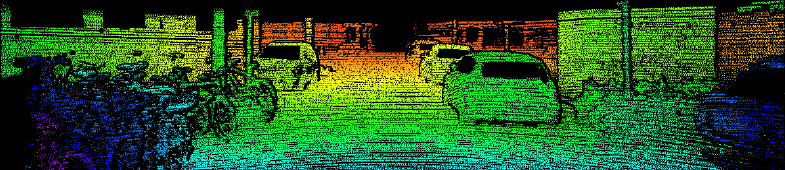
\includegraphics[width=\textwidth]{lidarGT}

  \note {
  \begin{itemize}
    \item Ground truth for a given frame is obtained by registering 5 consecutive frames before and after the one selected and accumulating the resulting point clouds.
    \begin{itemize}
      \item Ambiguous regions such windows and fences are manually removed
      \item The corresponding disparity map is computed using calibration information
    \end{itemize}
    \item The original benchmark also uses linear interpolation of missing values, making sparse and semi-dense methods comparable to dense ones -> This is not fair and hardly optimal // Worsened error metrics for non-dense algorithms.
    \item ... And not all the values
    \item To better understand the collected data, it will be plotted in a graph with the independent variable (x-axis) representing the measured value, and the dependent one (y-axis) the percentage of frames falling below it. Better-performing algorithms are those with a lower x value for a given frame percentage (e.g. y = 90%).
 \end{itemize}
 }
\end{frame}

\begin{frame}{Experimental setup}
  \framesubtitle{False correspondences estimation}
  \begin{itemize}
    \item A safety distance of about 1\,s is usually kept from a leading vehicle.
    \item A speed-dependent free volume is present in front of the ego-vehicle. \\
  \end{itemize}

  \begin{center}
    \begin{figure}[t]
	  \centering
	  \begin{subfigure}[t]{0.5\textwidth}
	      \includemovie[autoplay, repeat]{\linewidth}{0.5\textheight}{/home/nestor/Seafile/Videos/Tesis/cp03/FC.avi}
	  \end{subfigure}% 
	  ~
	  \begin{subfigure}[t]{0.5\textwidth}
	      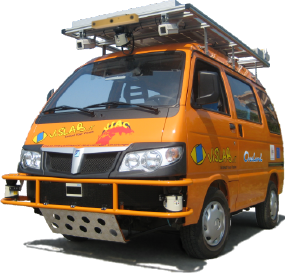
\includegraphics[height=0.5\textheight]{viac_van}
	  \end{subfigure}%       
    \end{figure}
  \end{center}

  \note {
    \begin{itemize}
     \item Any reconstructed point falling within said area must be considered as an erroneous estimate.
     \item We reject false negatives using the LIDAR information.
     \item Face correspondences percentage is the ratio of points inside the object-free volume respect to the total number of 3D points.
    \end{itemize}
  }
\end{frame}

\begin{frame}{Experimental setup}
  \framesubtitle{Normalized Cross Correlation (NCC)}

  \begin{center}
    \begin{figure}[t]
	  \centering
	  \begin{subfigure}[t]{0.5\textwidth}
	    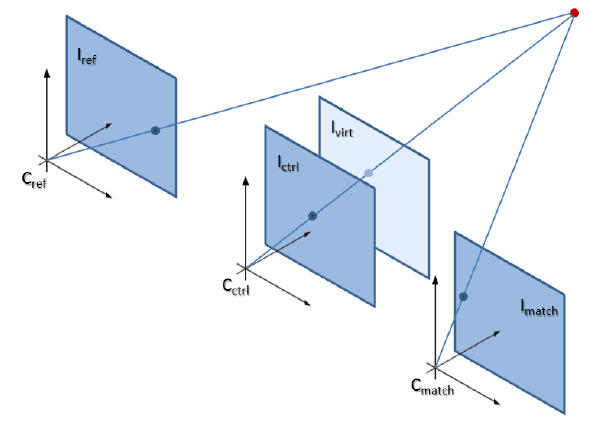
\includegraphics[width=\textwidth]{trinocular_setup}
	  \end{subfigure}% 
	  ~
	  \begin{subfigure}[t]{0.5\textwidth}
	    \includemovie[autoplay, repeat, controls]{\linewidth}{0.5\textheight}{/home/nestor/Seafile/Videos/Tesis/cp03/ncc.avi}	      
	  \end{subfigure}%       
    \end{figure}
  \end{center}

  \note {
    \begin{itemize}
     \item LIDAR-based GT takes time to be produced and FC is an indirect measurement.
     \item The use of a third camera allows to directly compare a reconstructed view with the actual images w/o manual intervention.

     \item NCC is calculated as described by Morales et al.

     \item It is suggested a configuration of 20 cm btween ref and match, and the ctrol camera is at 50 cm from ref camera
     \item In our conf, it is 24 and 12, respectively, as we use a precalibrated trinocular camera.
    \end{itemize}
  }
\end{frame}

\begin{frame}{Algorithms}
  Three dense reconstruction algorithms tested:
  \begin{itemize}
   \item Census Cost Semi-Global Matching (Census-SGM) \footnote{\cite{Hirschmuller2005, Hirschmuller2009}}
   \item Birchfield-Tomasi Semi-Global Matching (BT-SGM)\footnote{\cite{Hirschmuller2005, Birchfield1998}, \url{http://opencv.org}}
   \item Efficient Large-Scale Stereo Matching (ELAS) \footnote{\cite{Geiger2011}}
  \end{itemize}


  \note {
    \begin{itemize}
     \item LIDAR-based GT takes time to be produced and FC is an indirect measurement.
     \item The use of a third camera allows to directly compare a reconstructed view with the actual images w/o manual intervention.

     \item NCC is calculated as described by Morales et al.

     \item It is suggested a configuration of 20 cm btween ref and match, and the ctrol camera is at 50 cm from ref camera
     \item In our conf, it is 24 and 12, respectively, as we use a precalibrated trinocular camera.
    \end{itemize}
  }
\end{frame}

\begin{frame}{Algorithms}
  \framesubtitle{Semi-Global Matching}
  
  \begin{itemize}
    \item Disparity search range is reduced
    \begin{itemize}
      \item A set of sparse, robustly matched control points is found.
      \item A 2D mesh is generated via Delaunay triangulation.
      \item A prior is created from this mesh
    \end{itemize}
  \end{itemize}

  \note {
    By computing a piecewise linear function induced by the support point disparities and the triangulated mesh.
  }
\end{frame}

\begin{frame}{Algorithms}
  \framesubtitle{Efficient Large-Scale Stereo Matching (ELAS)}
  
  \begin{itemize}
    \item Gets the disparity map D by minimizing \\
    \begin{center} $E(D) = E_{data}(D) + E_{smooth}(D)$ \end{center}
    \item NP-complete (but tractable using DP).
    \item Two cost metrics:
    \begin{enumerate}
      \item Census cost metric.
      \begin{itemize}
	\item Hamming distance of the Census transform of a 5x5 window.
      \end{itemize}
      \item  Birchfield-Tomasi cost metric.
    \end{enumerate}
  \end{itemize}

  \note {
    \begin{itemize}
     \item $E_{data}$ is the pixel-wise matching cost
     \begin{itemize}
      \item Sum of all pixels matching costs for the disparities of D
     \end{itemize}
     \item $E_{smooth}$ is the smooth constraint.
     \begin{itemize}
      \item adds a small penalty P1 to all px in the neighborhood of a pixel p for which the disparity varies by one
      \item adds a higher penalty P2 if greater
     \end{itemize}
     \item SGM is no tractable in real time, unless we use a DP strategy
     \item each pixel is used as the px-wise matching function, instead of the mutual information, as used in the original implementation.
     \item Similar results, but reduces the overall processing burden
     \item Each position C(p, d) of the cost volume is initialized with the number of differing bits btween the corresponding transformed values of left-right images.
     \item We have used the freely available OpenCV implementation that uses BT pixel dissimilarity as cost metric to initialize the cost
    \end{itemize}
  }
\end{frame}

\begin{frame}{Algorithms}
\begin{table}[h!]
\begin{center}
\resizebox{\columnwidth}{!} {
\begin{tabular}{|l|c|c|c|c|c|}
 \cline{2-6}
 \multicolumn{1}{ c|}{} & \multicolumn{3}{ c| }{Census-SGM} &
 \multicolumn{1}{ c| }{\multirow{2}{*}{BT-SGM}} &
 \multicolumn{1}{ c| }{\multirow{2}{*}{ELAS}} \\ \cline{2-4}
 \multicolumn{1}{c|}{} & Config 1 & Config 2 & Config 3 & & \\ \cline{2-6}
 \hline \hline
 Gaussian filter & $\surd$ & $\surd$ & $\surd$ & - & - \\
 Sparse Census mask & - & - & - & - & - \\
 Ternarized Census & - & - & - & - & - \\
 Hamming scores aggregation  & - & - & - & - & - \\
 Uniqueness constraint & 10 & 20 & 20 & 10 & 15 \\
 Adaptive mean & $\surd$ & $\surd$ & $\surd$ & - & $\surd$ \\
 Despeckle filter & $\surd$ & $\surd$ & $\surd$ & $\surd$ & $\surd$ \\
 Gap filter & $\surd$ & $\surd$ & - & - & $\surd$ \\
 \hline \hline
 Other parameters & \multicolumn{3}{ |c }{$P_1=10$, $P_2=50$, L/R check} &
 \multicolumn{1}{ |c }{see \footnote{\url{http://www.cvlibs.net/datasets/kitti/eval\_stereo\_flow.php}}} &
 \multicolumn{1}{ |c| }{see \footnotemark[\value{footnote}]} \\
 \hline
\end{tabular}
}
\end{center}
\end{table}
\end{frame}


\subsection{Evaluation of Stereo 3D Reconstruction Algorithms}
\subsection{Stixel World}
\subsection{Particle Filter based Object Tracking}

\section{Obstacle Avoidance and Planning}
  \subsection{Global Planning}
  \subsection{Local Planning}
  
\section{Results}
  \subsection{Change Detection for Obstacle Localization in Images}
  \subsection{Non-Rigid Contour Tracking}
  \subsection{Evaluation of Stereo 3D Reconstruction Algorithms}
  \subsection{Stixel World}
  \subsection{Particle Filter based Object Tracking}
  \subsection{Global Planning}
  \subsection{Local Planning}
  
\section{Conclusions}
  \subsection{Future work}

% \section{Introducción}
%   \subsection{Modelos Basados en Adaptación Social}
%   
%   \begin{frame}
%     \frametitle{¿Qué es un modelo basado en adaptación social?}
%     \begin{definition}
%       Algoritmos o mecanismos distribuidos de resolución de problemas inspirados en el comportamiento colectivo de colonias de insectos sociales u otras  sociedades de animales.
%     \end{definition}
%     \begin{example}
%       \begin{itemize}
%       \item <1->Insectos
%       \item <2->Aves \pause
%       \item <3->Peces \pause
%       \item <4->Mamíferos
%       \end{itemize}
%     \end{example}
%   \end{frame}
%   
% \section{Algoritmos de ejemplo}
%   \subsection{Optimización de colonia de hormigas}
% 
%   \begin{frame}
%     Algo de texto
%   \end{frame}
% 
%   \subsection{Difusión estocástica}
%   \begin{frame}
%     Algo de texto
%   \end{frame}
% 
%   \section{Aplicaciones}
%   \begin{frame}
%     Algo de texto
%   \end{frame}
  

%   \begin{frame}
%   \includemovie[
%     poster,
%     text=(/tmp/M2U00318.MPG),
%     mouse,
%     repeat
%     ]{
%     .5\linewidth
%     }{
%     .375\linewidth
%     }{/tmp/M2U00318.MPG}
%   \end{frame}
  
\end{document}
